\chapter{Using network analysis to examine co-occurrence patterns of animal pest injuries and diseases in farmers' fields in different production environments in South and South East Asia}

\subsection{Introduction}

Agricultural crop plants are frequently injured, or infected by more than one species of pests and pathogens at the same time. Many of these injuries may affect yields. Because of this co-occurrence in injuries, the idea of ``crop health" has been highlighted and implemented to manage the combination of injuries or so-called injury profiles \citep{Savary_2006_Quantification}. Co-occurrence patterns of injuries are beginning to provide important insight into these injury profiles, which possibly present co-occurring or anti-co-occurring (mutually exclusive) relationships between injury-injury. Uncovering these patterns is important to implications in plant disease epidemiology and management. However, there are only a few reports of injury–injury relationships in rice crop systems are currently unknown. This could be a difficult task since complex patterns of injury profiles are related to environmental conditions, cultural practices, and geography \citep{Willocquet_2008_Simulating}.

To address this issue, we used in-field surveys as a tool to develop ground-truth databases that allowed us to identify the major yield reducing pests in irrigated lowland rice ecosystems. These sorts of databases provide an overview of the complex relationships between crop, field management, pest injuries, and yields. Several previous studies \citet{Savary_2000_Quantification, Savary_2000_Characterization, Dong_2010_Characterization} and \citet{Reddy_2011_Characterizing} involved surveys that were used to characterize injury profiles in an individual production situation (a set of factors including cultural practices, weather condition, socioeconomics, \textit{etc}.) that determine agricultural production, and the injury profiles using nonparametric multivariate analysis such as cluster analysis, correspondence analysis, or multiple correspondence analysis. Their results led to the conclusions that injury profiles (the combination of disease and pest injury that may occur in a given farmer’s field) were found co-occurrence patterns across sites, which are associated at regional scale. For example, stem rot, sheath blight, planthopper, and rice whorl maggot injuries, are high incidence, with low incidence of brown spot, and absence of bacterial leaf blight, leaf blast, and neck blast are a common pattern in tropical Asia from the study of \citet{Savary_2000_Characterization}.

Co-occurrence analysis and network theory have recently been used to reveal the patterns of co-occurrence between microorganisms in the complex environments ranging from human gut to ocean and soils \citep{Faust_2012_Microbial_co, Ma_2016_Geographic}. Co-occurrence patterns are ubiquitous and particularly important in understanding community structure, offering new insights into potential interaction in networks. Recent reviews of network based approaches revealed that these tools have demonstrated previously unseen co-occurrence patterns, such as strong non-random association, topology based analysis of large networks has been proven powerful for studying the characteristics of co-occurrence pattern of the communities in ecological community \citep{Williams_2014_demonstrating, Barberan_2012_Network}, or key actors in social networks \citep{Crowston_2006_Hierarchy}. Here, we significantly advance this study by providing a comprehensive understanding of the topological shifts of animal pest injury and disease co-occurrence networks at regional scale.

South and Southeast Asia represent big bowl of rice for the world population. Comparing the topological properties of the node associated with occurrence in the different countries and examining network level topological features can provide us with insight into variation in the co-occurrence patterns of rice injuries in different countries. This approach helps contextualize the animal pests -- disease association by taking to account the complex network of potential association among animal pest and disease occurring in farmers’ fields in these countries. Specifically, we addressed the following questions:(i) How can the co-occurrence relationships of rice injuries be examined from the perspective of network analysis (ii) Which animal injuries and diseases are found commonly close co-occurrence patterns among other variables in order to target to control or monitor. To answer these questions, we performed crop health survey at the farmers’ fields in two different seasons and five countries in South and Southeast Asia and implemented co-occurrence network analysis to examine the topological feature differences across countries. The main objective was to characterize and better understand co-occurrence networks in the association of rice animal pest injuries and diseases.

\subsection{Materials and methods} 

I designed a statistical approach written in R v. 3.0.1 \citep{R_2015}. All scripts necessary to replicate this analysis are included in the appendix. The analysis presented in this chapter is designed to contract network models of co-occurrence patterns of rice injuries at different levels across cropping seasons (wet, and dry season), and production environments. I considered co-occurrence to be positive rank correlations coefficients ($\rho$ from the Spearman’s correlation at $p$-value < 0.05) between pairs of injures within each dataset with the strength of the relationship represented by the correlation coefficient. 

\subsubsection{Network construction}

The co-occurrence network was inferred based on the Spearman correlation matrix constructed with \texttt{R} function \texttt{cor.test} with parameter method `Spearman' (package stats) was used for calculate Spearman's correlation coefficient ($\rho$), which is defined as the Pearson correlation coefficient between the ranked variables \citep{R_2015}. Nodes in this network represent injuries and the edges that connect these nodes represent correlations between injuries. Based on correlation coefficients and $p$-values for correlation, we constructed co-occurrence networks. The cutoff of $p$-values was 0.05.  The networks were visualized with \textbf{igraph} package \citep{Csardi_2010_igraph} using directed network and the Fruchterman–Reingold layout \citep{Fruchterman_1991_Graph}. Network properties were calculated with the \textbf{igraph} package.

\subsubsection{Topological feature analysis}

I calculated the topological features of each network using \textbf{igraph} package. To describe the topology of the resulting networks, a set of measures (node degree, betweenness, local clustering coefficient, average clustering coefficient, and average path length) were calculated \citep{Newman_2006_Modularity}. Node degree is measured by the number of the edges (connections) of a node has. Betweenness of a node is defined by the number of of shortest paths going through a node, and the local clustering coefficients of a node is the ratio of existing edges connecting a node's neighbors to each other to the maximum possible number of such edges. Average clustering coefficient, and average path length were measured for each network. The network clustering coefficient measures the degree to which nodes of the network tend to cluster together and is a measure of the connectedness of the network and is indicative of the degree of relationships in the network. Average path length is the average number of steps along the shortest paths for all possible pairs of network nodes, and diameter is the greatest distance between any pair of nodes. 


The average clustering coefficient is defined as:
\begin{equation}
C = \frac{3 \times \mbox{number of triangles}}{\mbox{number of connected triplets of vertices}} = \frac{\mbox{number of closed triplets}}{\mbox{number of connected triplets of vertices}}.
\end{equation}

The average short path is defined as:
\begin{equation}
l_G = \frac{1}{n \cdot (n - 1)} \cdot \sum_{i \ne j} d(v_i, v_j)
\end{equation}

Node were further classified by ranking all nodes according to three node features, partitioning this ranked list into three equally value of each node property. Nodes with high rank value in top third proportion of node degree, and high rank value in top third proportion of betweenness are recognized as indicator in co-occurrence network of rice injuries. 


\subsubsection{Community detection}

Modularity reflects the degree to which a network is organized into a modular or community structure. Modules refer to a set of nodes with denser links among them but sparser links with the rest of the network \citep{Newman_2006_Modularity}. Detection and characterization of modular structure in rice injury co-occurrence can help us to identify groups of injuries that closely related and often (but not always) occur together under same situation. Several optimization algorithms are currently available, each with different advantages \citep{Brandes_2008_Modularity}. Based on the identified community structure, nodes can be grouped in terms of their roles in maintaining intra or inter-module connectivity. In this chapter, the network was detected the community structures by maximizing the modularity measure over all possible partitions by using \texttt{cluster\_optimal} function of \textbf{igraph} package.

\subsection{Result}
I used crop heath survey data

\textbf{Prevalence of injuries across sites and seasons}
In the previous chapter, 
Differences among sites and seasons for injury prevalence (percent fields affected by a given injury) were summarized (Table 3).

%In our analysis, both diameter and average path length are considered measures of the size of the network. Larger networks are less connected, meaning that the likelihood of a strong connection between any two randomly selected species is low. The network clustering coefficient are considered measures of the complexity of the network. The networks are more complex, the network has higher clustering coefficient, and shorter average path length.

 Among the injuries caused by pathogens, SHB showed the highest prevalence, exceeding 50\% in any site–season combination. SHR, BS, and SR occurred in decreasing order of prevalence level. At the other end of this spectrum, RTD was observed in one site and one season only, and thus was not further considered in the analyses. Insect injuries appear to have higher prevalence than those due to pathogens. Most insect injuries were omnipresent, often with prevalence exceeding 80\%.

The injuries caused by animal pests observed during the survey period were rat injury (RT), deadheart (DH) and whitehead (WH) caused by stem borers, whorl maggot injury (WM), leaffolder injury (LF), gall midge injury or silver shoot (GM). Rat injuries were observed at all 5 survey locations with low incidence (less than 20\% incidence). We could observe 75\% incidence of the rat injury in MKD in dry season. They were also observed at WJV in dry season, and both season in TMN, LAG, SPB. Gall midge injuries during survey period were not observed in TMN and LAG, but it was found in SPB, MKD, but WJV at 25 \% incidence. Deadheart were observed all survey sites, and it was severe in dry season at SPB and MKD, but in WJV and LAG, it was severe in dry season. The trend of whitehead incidences observed was opposite the deadheart incidence, which whitehead incidences were more server in wet season at SPB and MKD, but less severe at WJV and LAG. Leaffolder injury was observed all survey locations. The leaffolder incidences were more severe in wet season the dry season at WJV, TMN, and LAG. As apposite to SPB and MKD, they were more severe in dry season than wet season. Whorl maggot injury was observed at all locations. Mostly, they were more severe in wet season than dry season at all surveyed locations, except LAG.

Rice diseases recorded were bacterial leaf blight (BLB), bacterial leaf streak (BLS), brown spot (BS), leaf blast (LB), narrow brown spot (NBS), read stripe (RS), sheath blight (SHB), sheath rot (SR), false smut (FS), stem rot (SR). Rice diseases we observed in this study were commonly found at all locations, but there were some diseases that could not find especially in TMN such as BLS, BS, NBS, DP, RS, SHR, and SR. BLB was observed all location. BLB incidence was higher in dry season than wet season in WJV and MKD except in TMN, LAG, SPB. Wet season was more favorable for BLS than dry season because the incidence was higher in wet season than dry season. As same as BLS, BS incidence was higher in wet season than dry season, and it was severe in SPB. Even though, LB is common disease in these survey locations, but there were some farmer’s fields observed LB. In WJV and MKD, the LB incidence was higher in dry than wet season season. There were many field in SPB found high level of NBS incidence. Like BLS and BS, NBS incidence was more severe in wet season than dry season. There were many fields found high RS incidences. The highest incidences of DP were found in MKD. FS were commonly found at all location. The high incidents were observed in SPB, and MKD. NB were observed at all location. They were found many observations in TMN.  SHB commonly was found all location, and high incidence was in TMN, and LAG. 

Rice bug (RB) could be observed all survey location. They were highly found in dry season than wet season at WJV, LAG, and MKD. but in SPB, they were found only in wet season during the survey period.  Green leafhoppers were observed all location. They were found in LAG higher than other locations.

\subsubsection{Communities, Structures and compositions of co-occurrence network of rice pest injuries}
I should review or descript how to interpret network model 
\ref{table:network_prop}
\paragraph{Central Plain, Thailand}

Dry season network (Fig \ref{fig:networkCP_ds}) was composed of 18 associated injuries and captured 60 associations (edges). The network showed two groups of injury syndromes (the combination of injuries) based on the optimal clustering algorithm. The group1 (green) was more closely clustered than another group, according to node properties, the injuries in group1 had high clustering coefficient such as WH, SHR, SHB, DP, BS, RH, NB, DH, FS, HB, and RS. This indicated that these injuries formed complex co-occurrence relationships. Network properties (table \ref{table:nodepropCP_ds}) showed that WM and LF, BS, BLB, NBS are high-betweenness nodes.  As opposed to other injuries, LB and BLS had low scores on two from three centrality measure. Apparently, LB less possibly co-occur with other injuries (low betweenness), and did not co-occur with other injuries (low degree and clustering coefficient).

In wet season, the co-occurrence patterns of rice injuries had 4 syndromes (groups).  Fig \ref{fig:networkCP_ws} showed 8 injuries and ??  significant relationships (edges). Group3 (purple) is composed of BLS, RS, HB, SHB, SHR and WM. They were closer to each other than other groups based on the structure and clustering coefficient(table \ref{table:nodepropCP_ws}). The members of this group such as WM, HB, SHB, RS also had high node degree, which indicated that when they occurred, injuries in group2 (orange) tend to occur because of their associations. Group4 (pink) connected to group3 only, so the injuries in group4 depended on the injuries of groupd3, and were less likely to occur in this season.  RT and RB were less likely to occur in this season because of low centrality, if they presented in rice fields, other injuries had low tendency to occur. 

\begin{figure}
    \centering
    \begin{subfigure}[b]{1\textwidth}
        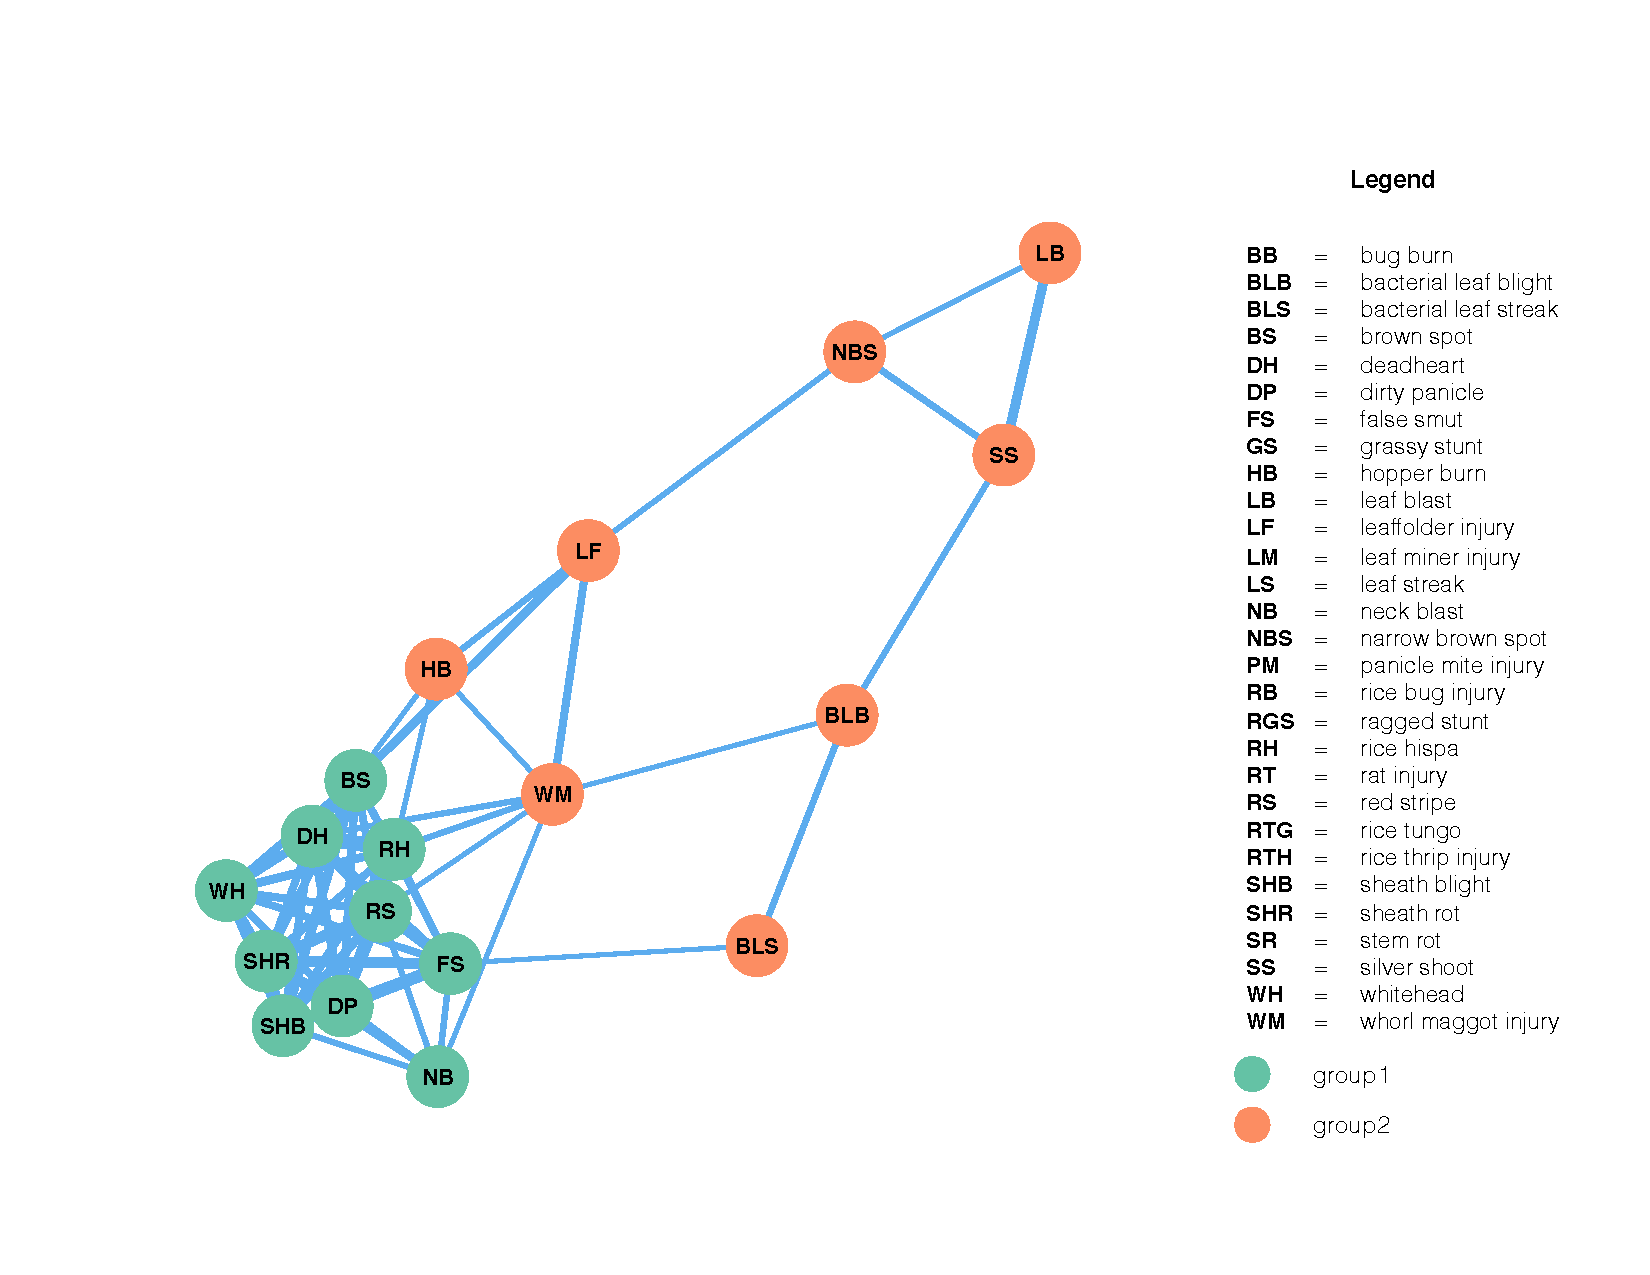
\includegraphics[width = 1\textwidth]{figures/networkCP_ds/networkCP_ds.pdf}
        \caption{Co-occurrence network of rice injuries in dry season at Central Plain, Thailand. The layout of the network graph is based on the Fruchterman-Reingold algorithm, which places nodes with stronger or more connections closer to each other.}
        \label{fig:networkCP_ds}
    \end{subfigure}
    \begin{subfigure}[b]{1\textwidth}
        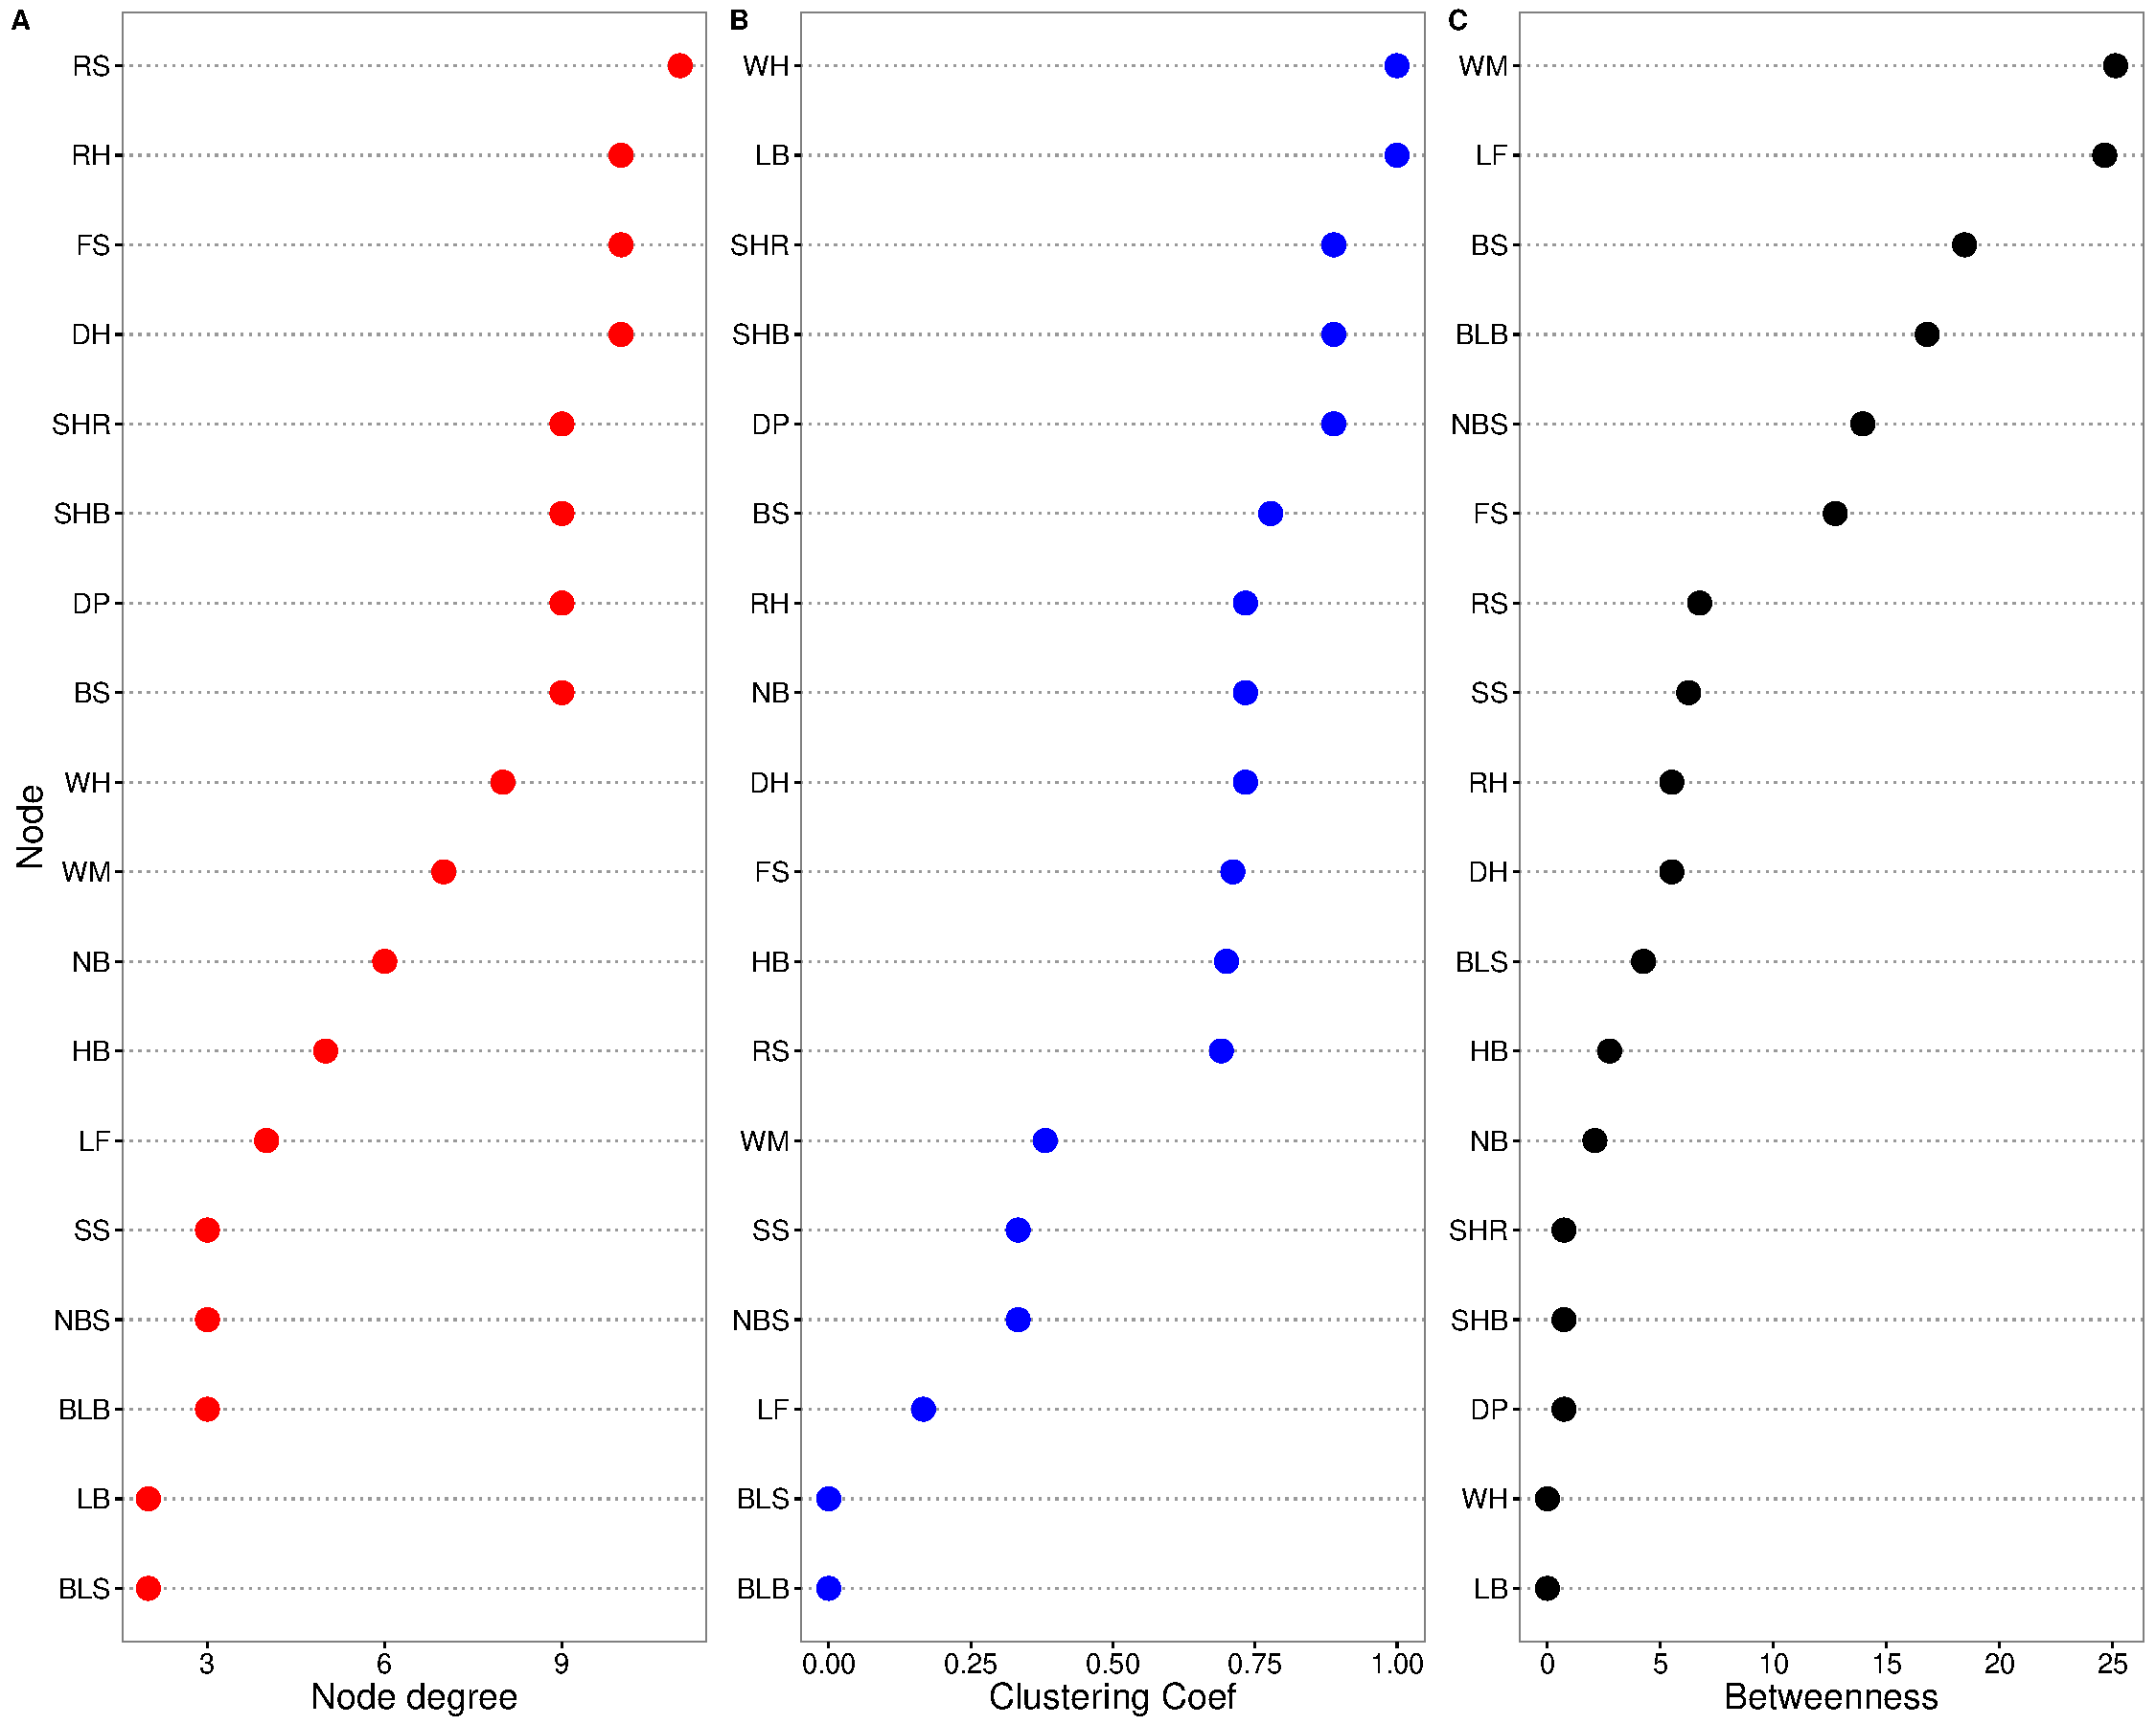
\includegraphics[width = 1\textwidth]{figures/nodepropCP_ds/nodepropCP_ds.pdf}
        \caption{Three centrality measures of the nodes in co-occurrence network of rice injuries in dry season at Central Plain. A: node degree, B:clustering coefficient, and C:Betweenness.}
        \label{fig:nodepropCP_ds}
    \end{subfigure}
    \caption{Rice injuries in dry season in Central Plain, Thailand}
    \label{fig:CP_ds}
\end{figure}

\begin{figure}
    \centering
    \begin{subfigure}[b]{1\textwidth}
        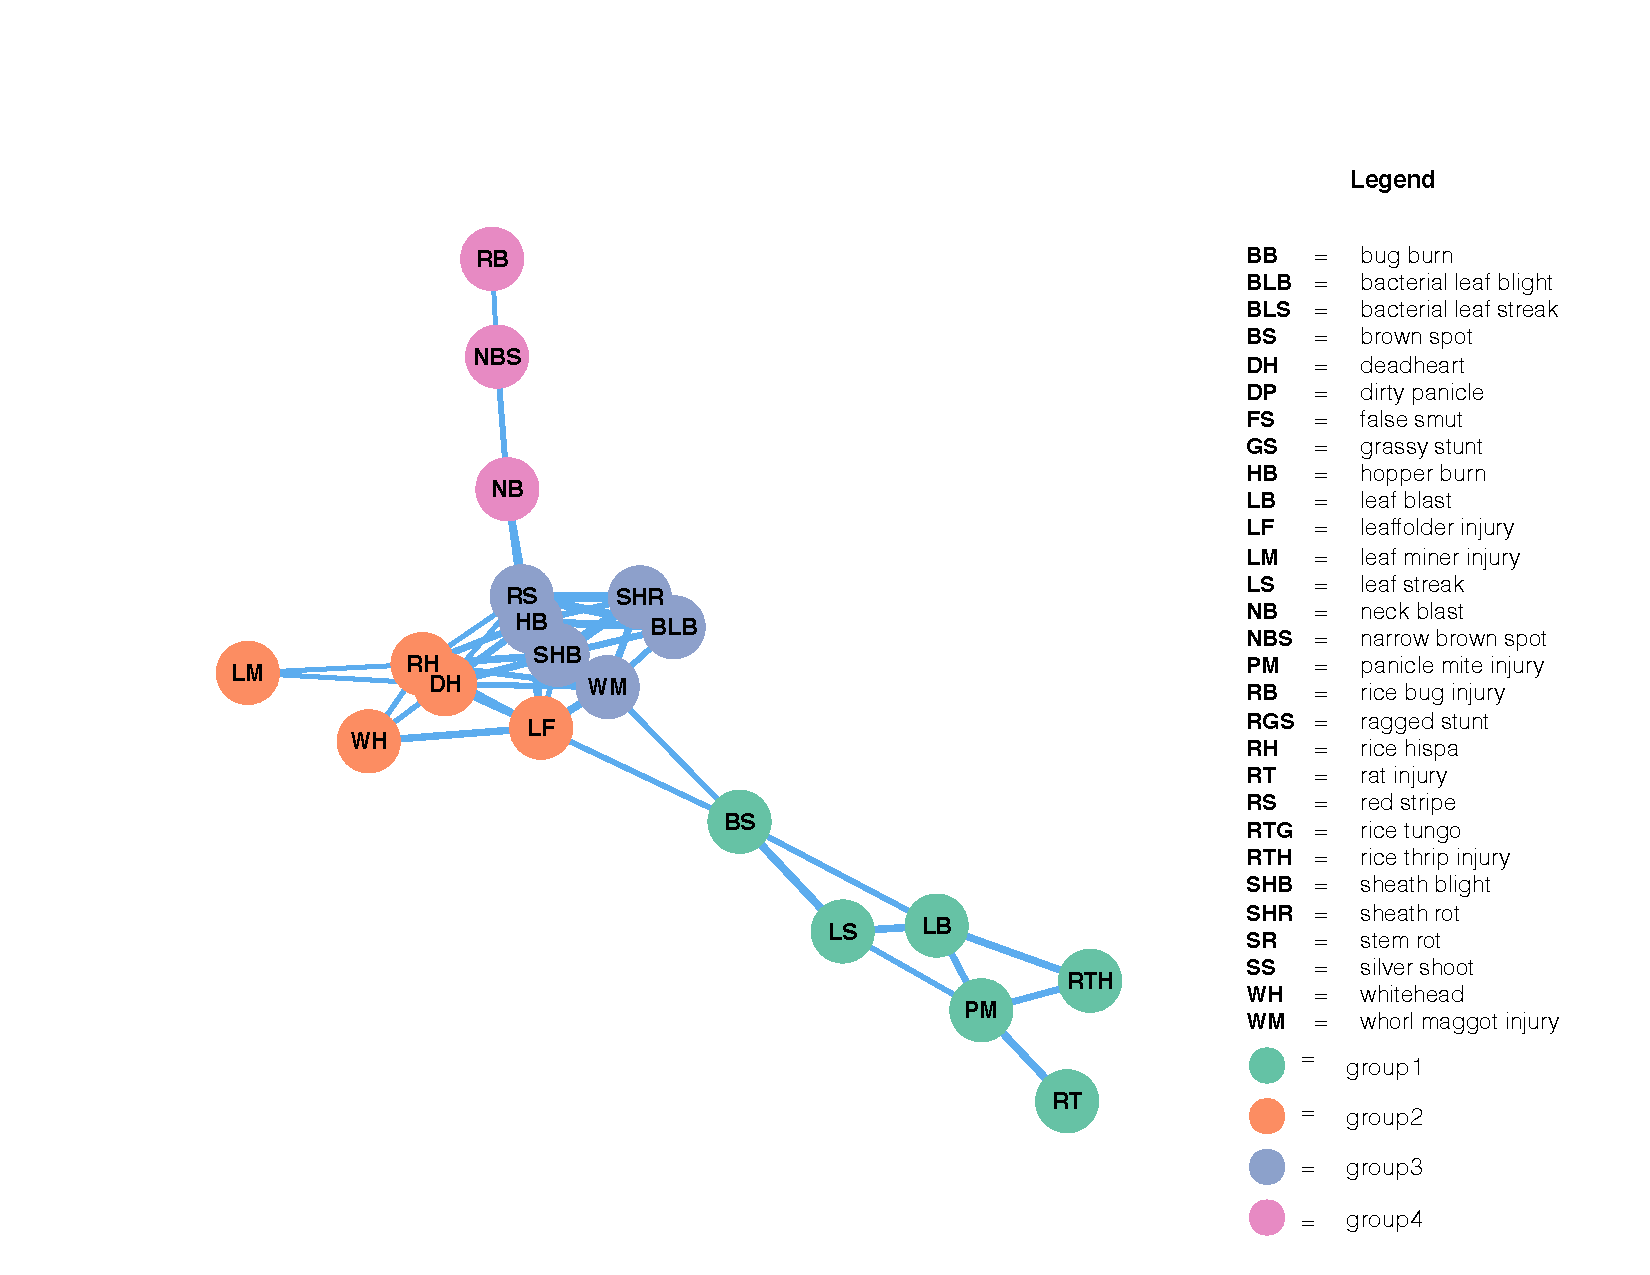
\includegraphics[width = 1\textwidth]{figures/networkCP_ws/networkCP_ws.pdf}
        \caption{Co-occurrence network of rice injuries in dry season at Central Plain, Thailand. The layout of the network graph is based on the Fruchterman-Reingold algorithm, which places nodes with stronger or more connections closer to each other.}
        \label{fig:networkCP_ws}
    \end{subfigure}
    \begin{subfigure}[b]{1\textwidth}
        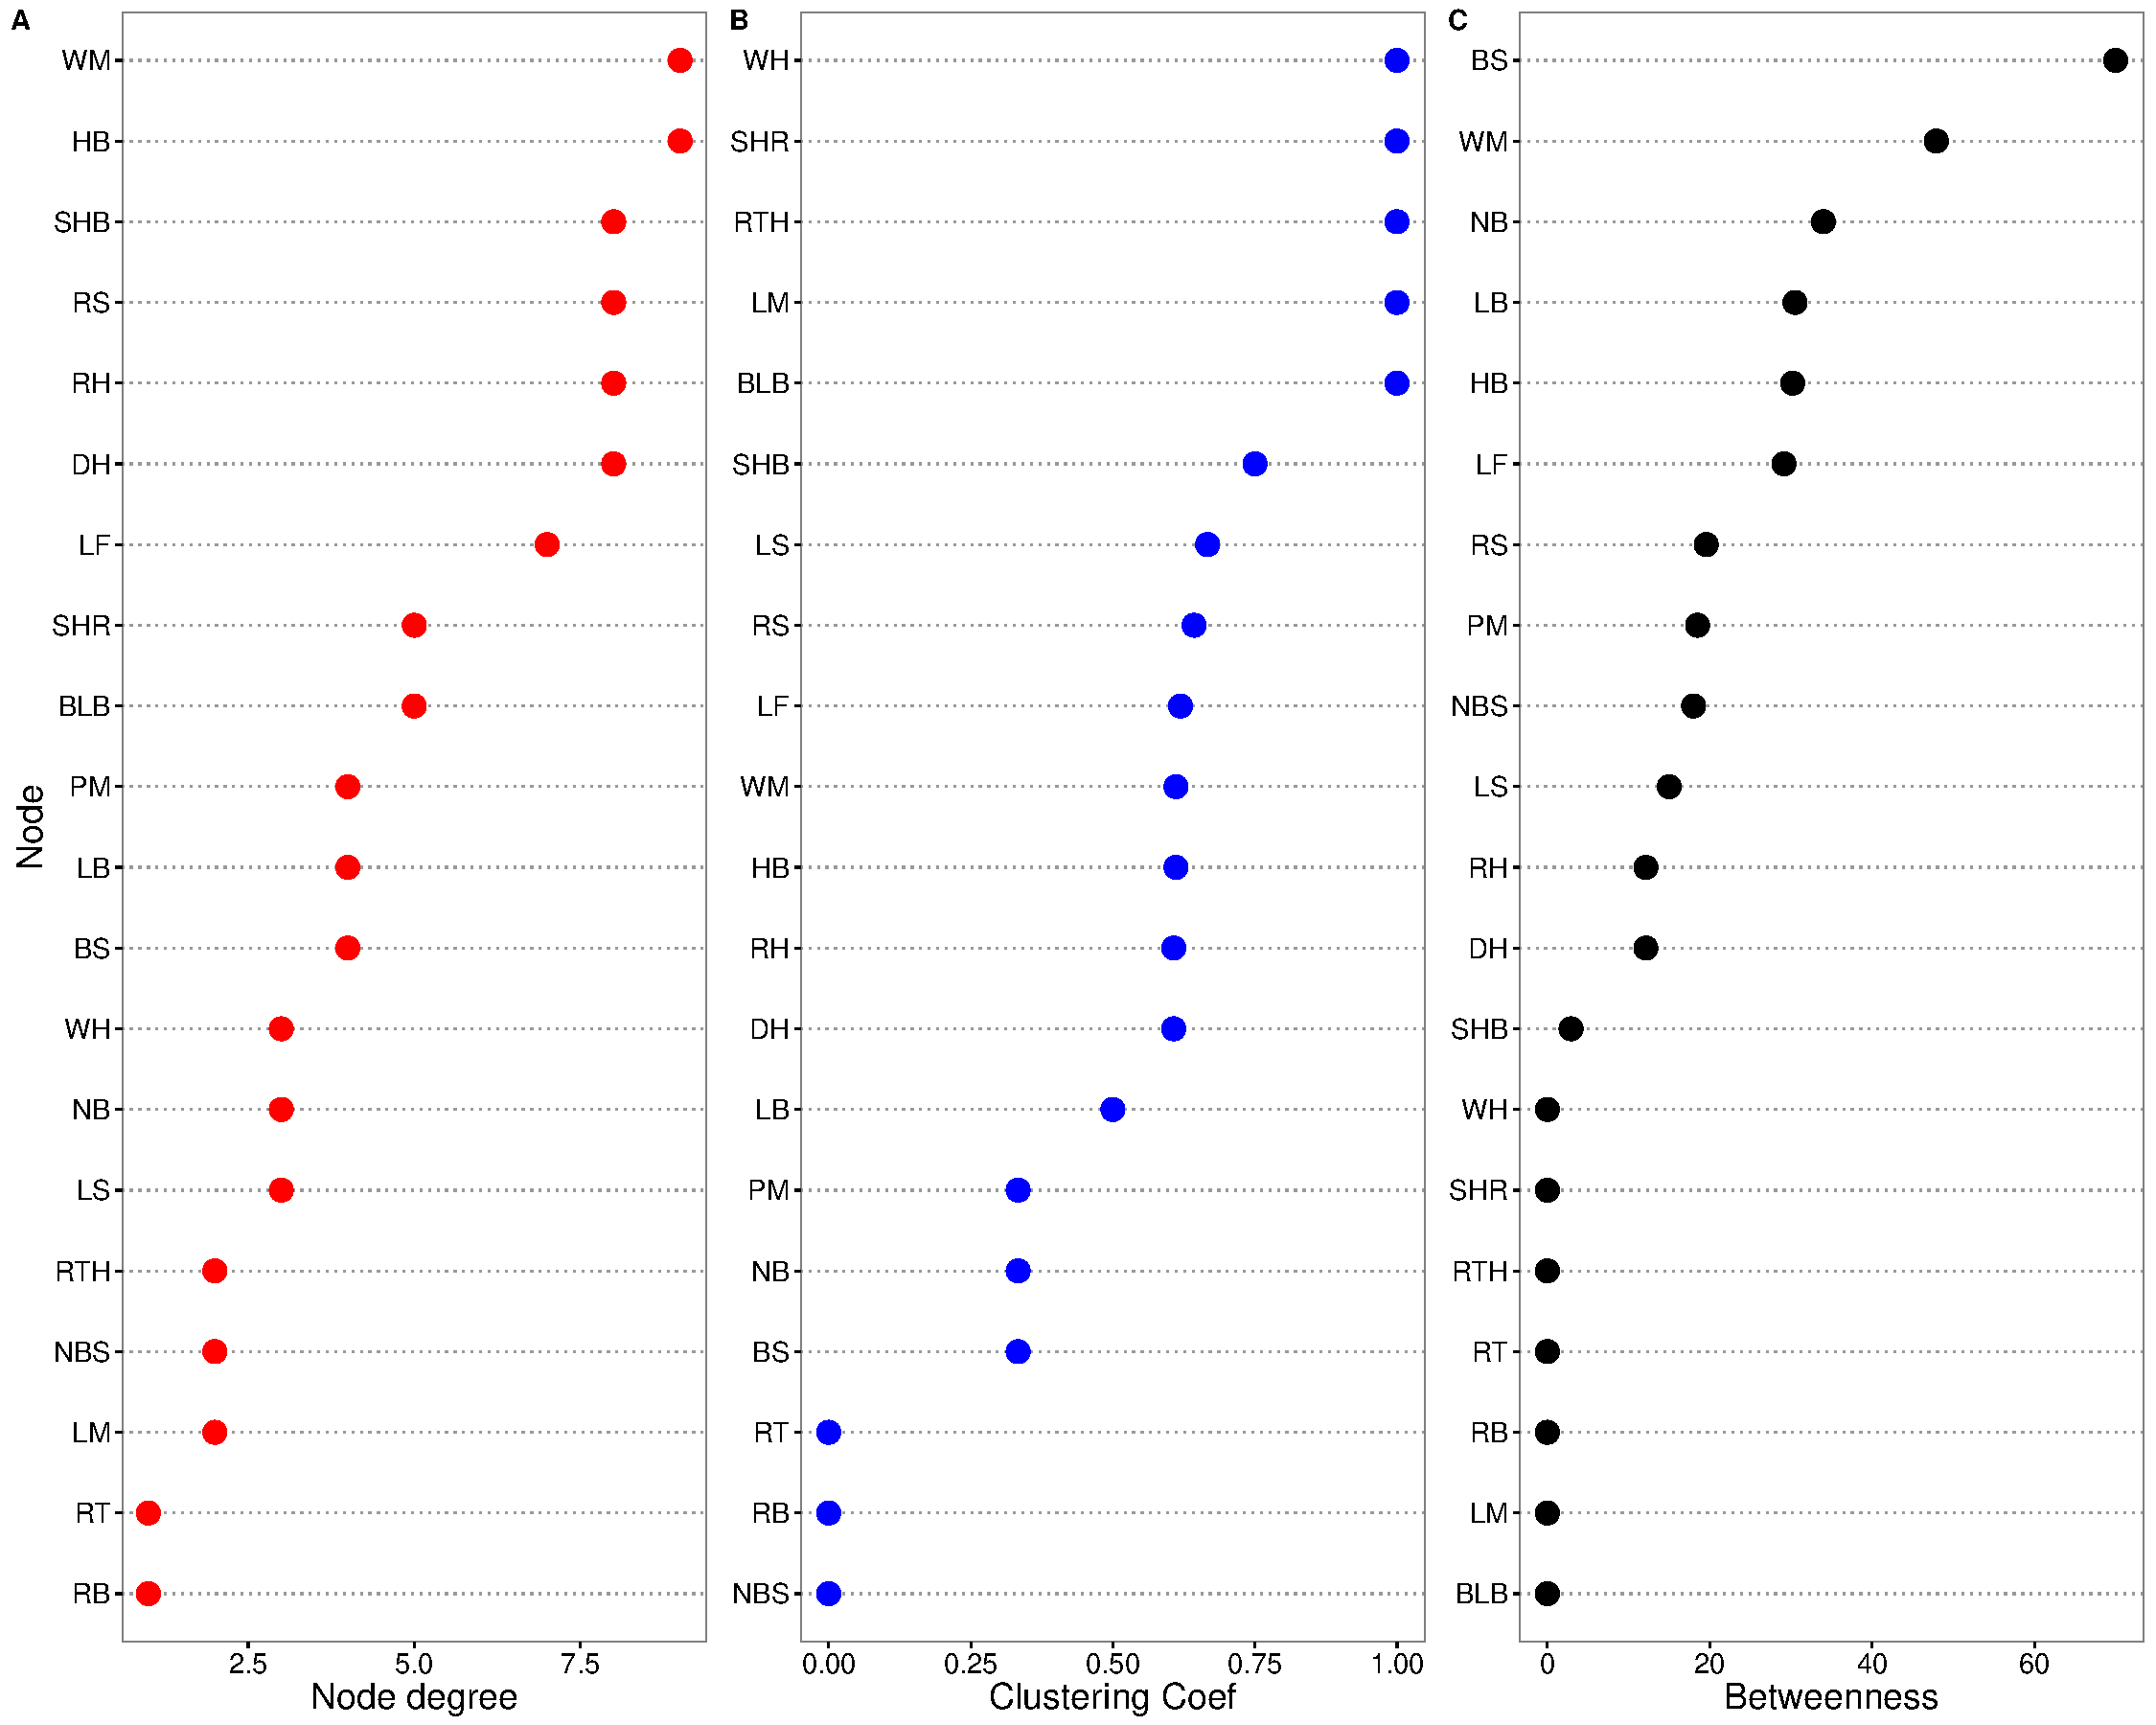
\includegraphics[width = 1\textwidth]{figures/nodepropCP_ws/nodepropCP_ws.pdf}
        \caption{Three centrality measures of the nodes in co-occurrence network of rice injuries in dry season at Central Plain. A: node degree, B:clustering coefficient, and C:Betweenness}
        \label{fig:nodepropCP_ds}
    \end{subfigure}
    \caption{Injuries in Central Plain, Thailand}
    \label{fig:CP_ws}
\end{figure}

\paragraph{Odisha, India}

Co-occurrence network of rice injuries in dry season (Figure \ref{fig:networkOR_ds}) was composed of ?? associated injuries and captured ?? associations. The network showed two isolated groups of injuries. Injuries within groups were closely related based on clustering coefficient (Table \ref{table:nodepropOR_ds}). This network could be inferred that there are two injury syndromes. One was the combination of BS, BLB, WM and SHB. Another was RH, WH, DH, LB, NB.

The network in wet season (Figure \ref{fig:networkOR_ws}) was more complex than dry season one. It composed of ?? nodes with ?? edges. The network reveals four groups of injury profiles. Group4 was isolated from the rest. Group2 was the biggest group placed in the middle of group1 and 3. The injuries in group2 had high node degree (table \ref{table:nodepropOR_ws}), which mean they were connected to many injuries. NBS and LF, injuries in group1 and group2, respectively presented high betweenness values and connected to injuries of group3. This indicated that group3 injuries had high chance to occur together with group1 and 2, but not group4. 

\begin{figure}
    \centering
    \begin{subfigure}[b]{1\textwidth}
        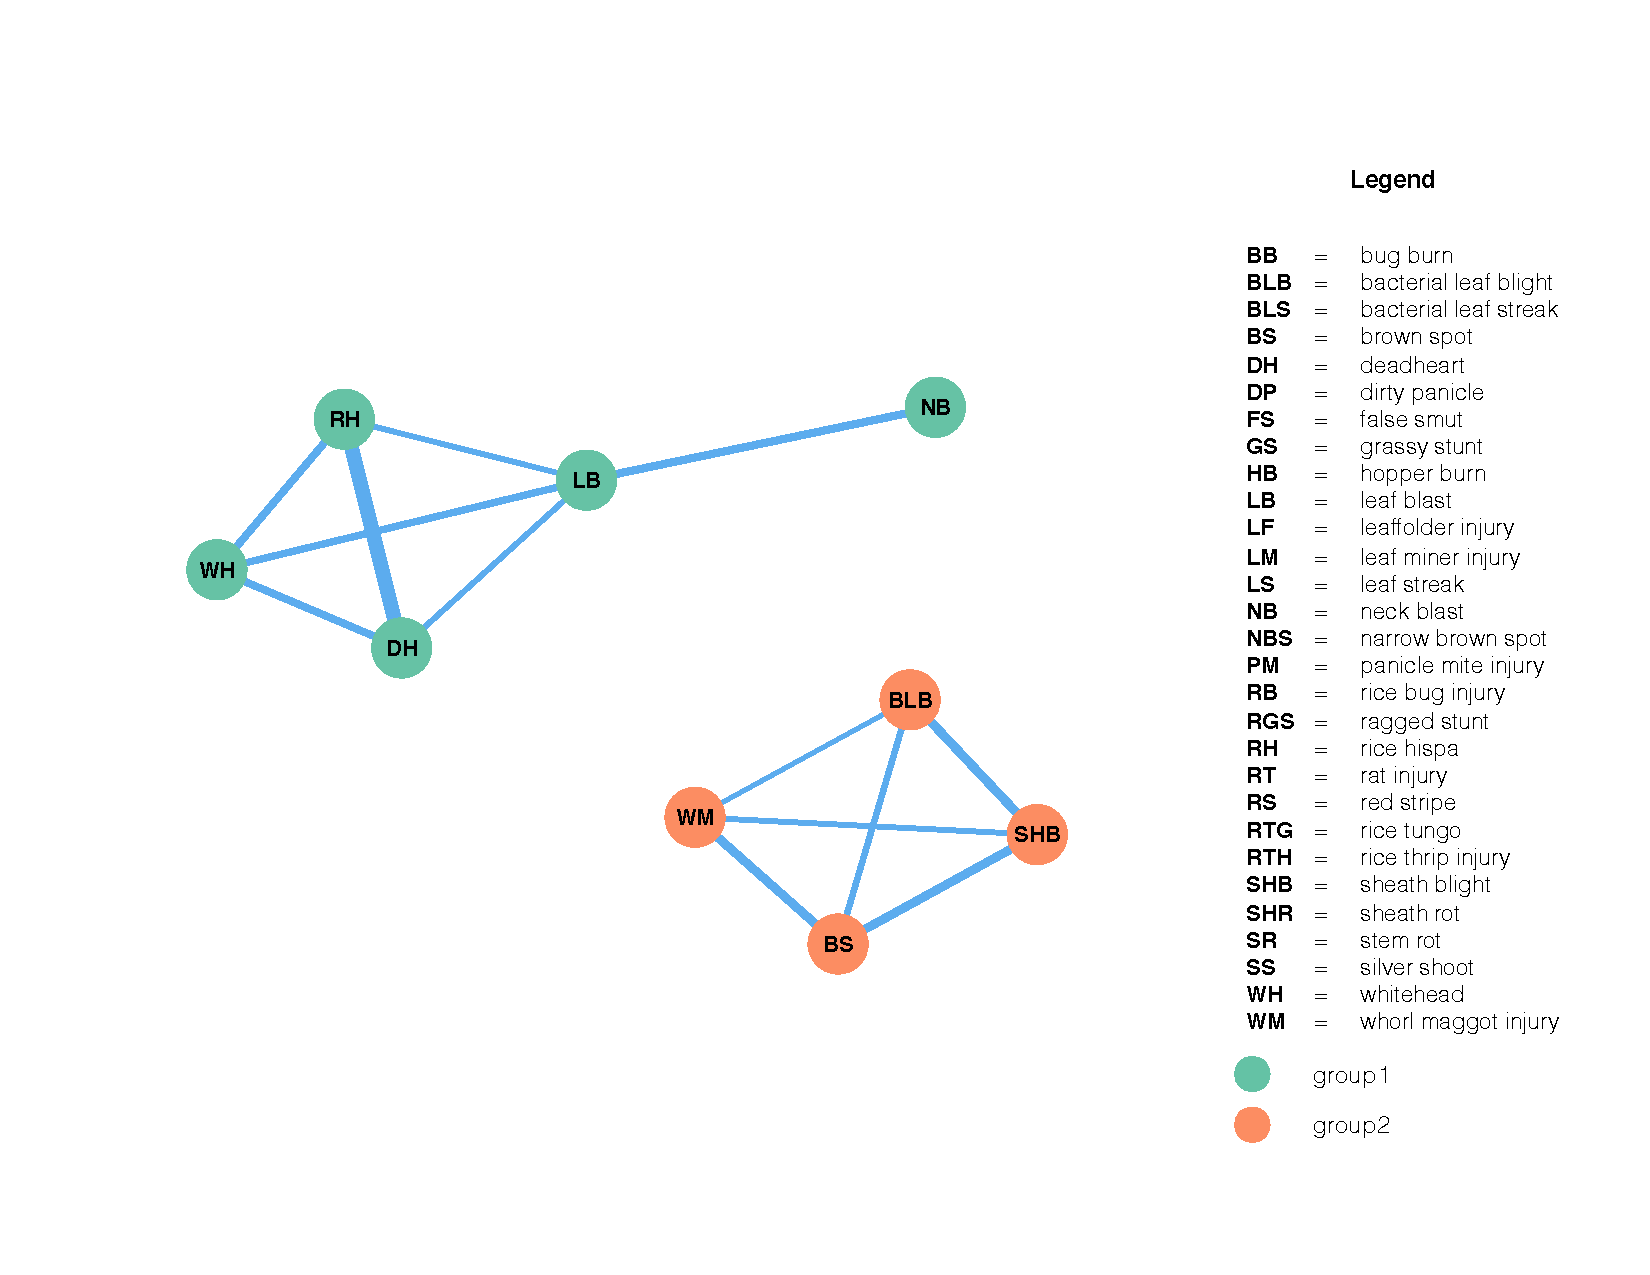
\includegraphics[width = 1\textwidth]{figures/networkOR_ds/networkOR_ds.pdf}
        \caption{Co-occurrence network of rice injuries in wet season at Odisha, India. The layout of the network graph is based on the Fruchterman-Reingold algorithm, which places nodes with stronger or more connections closer to each other.}
        \label{fig:networkOR_ds}
    \end{subfigure}
    \begin{subfigure}[b]{1\textwidth}
        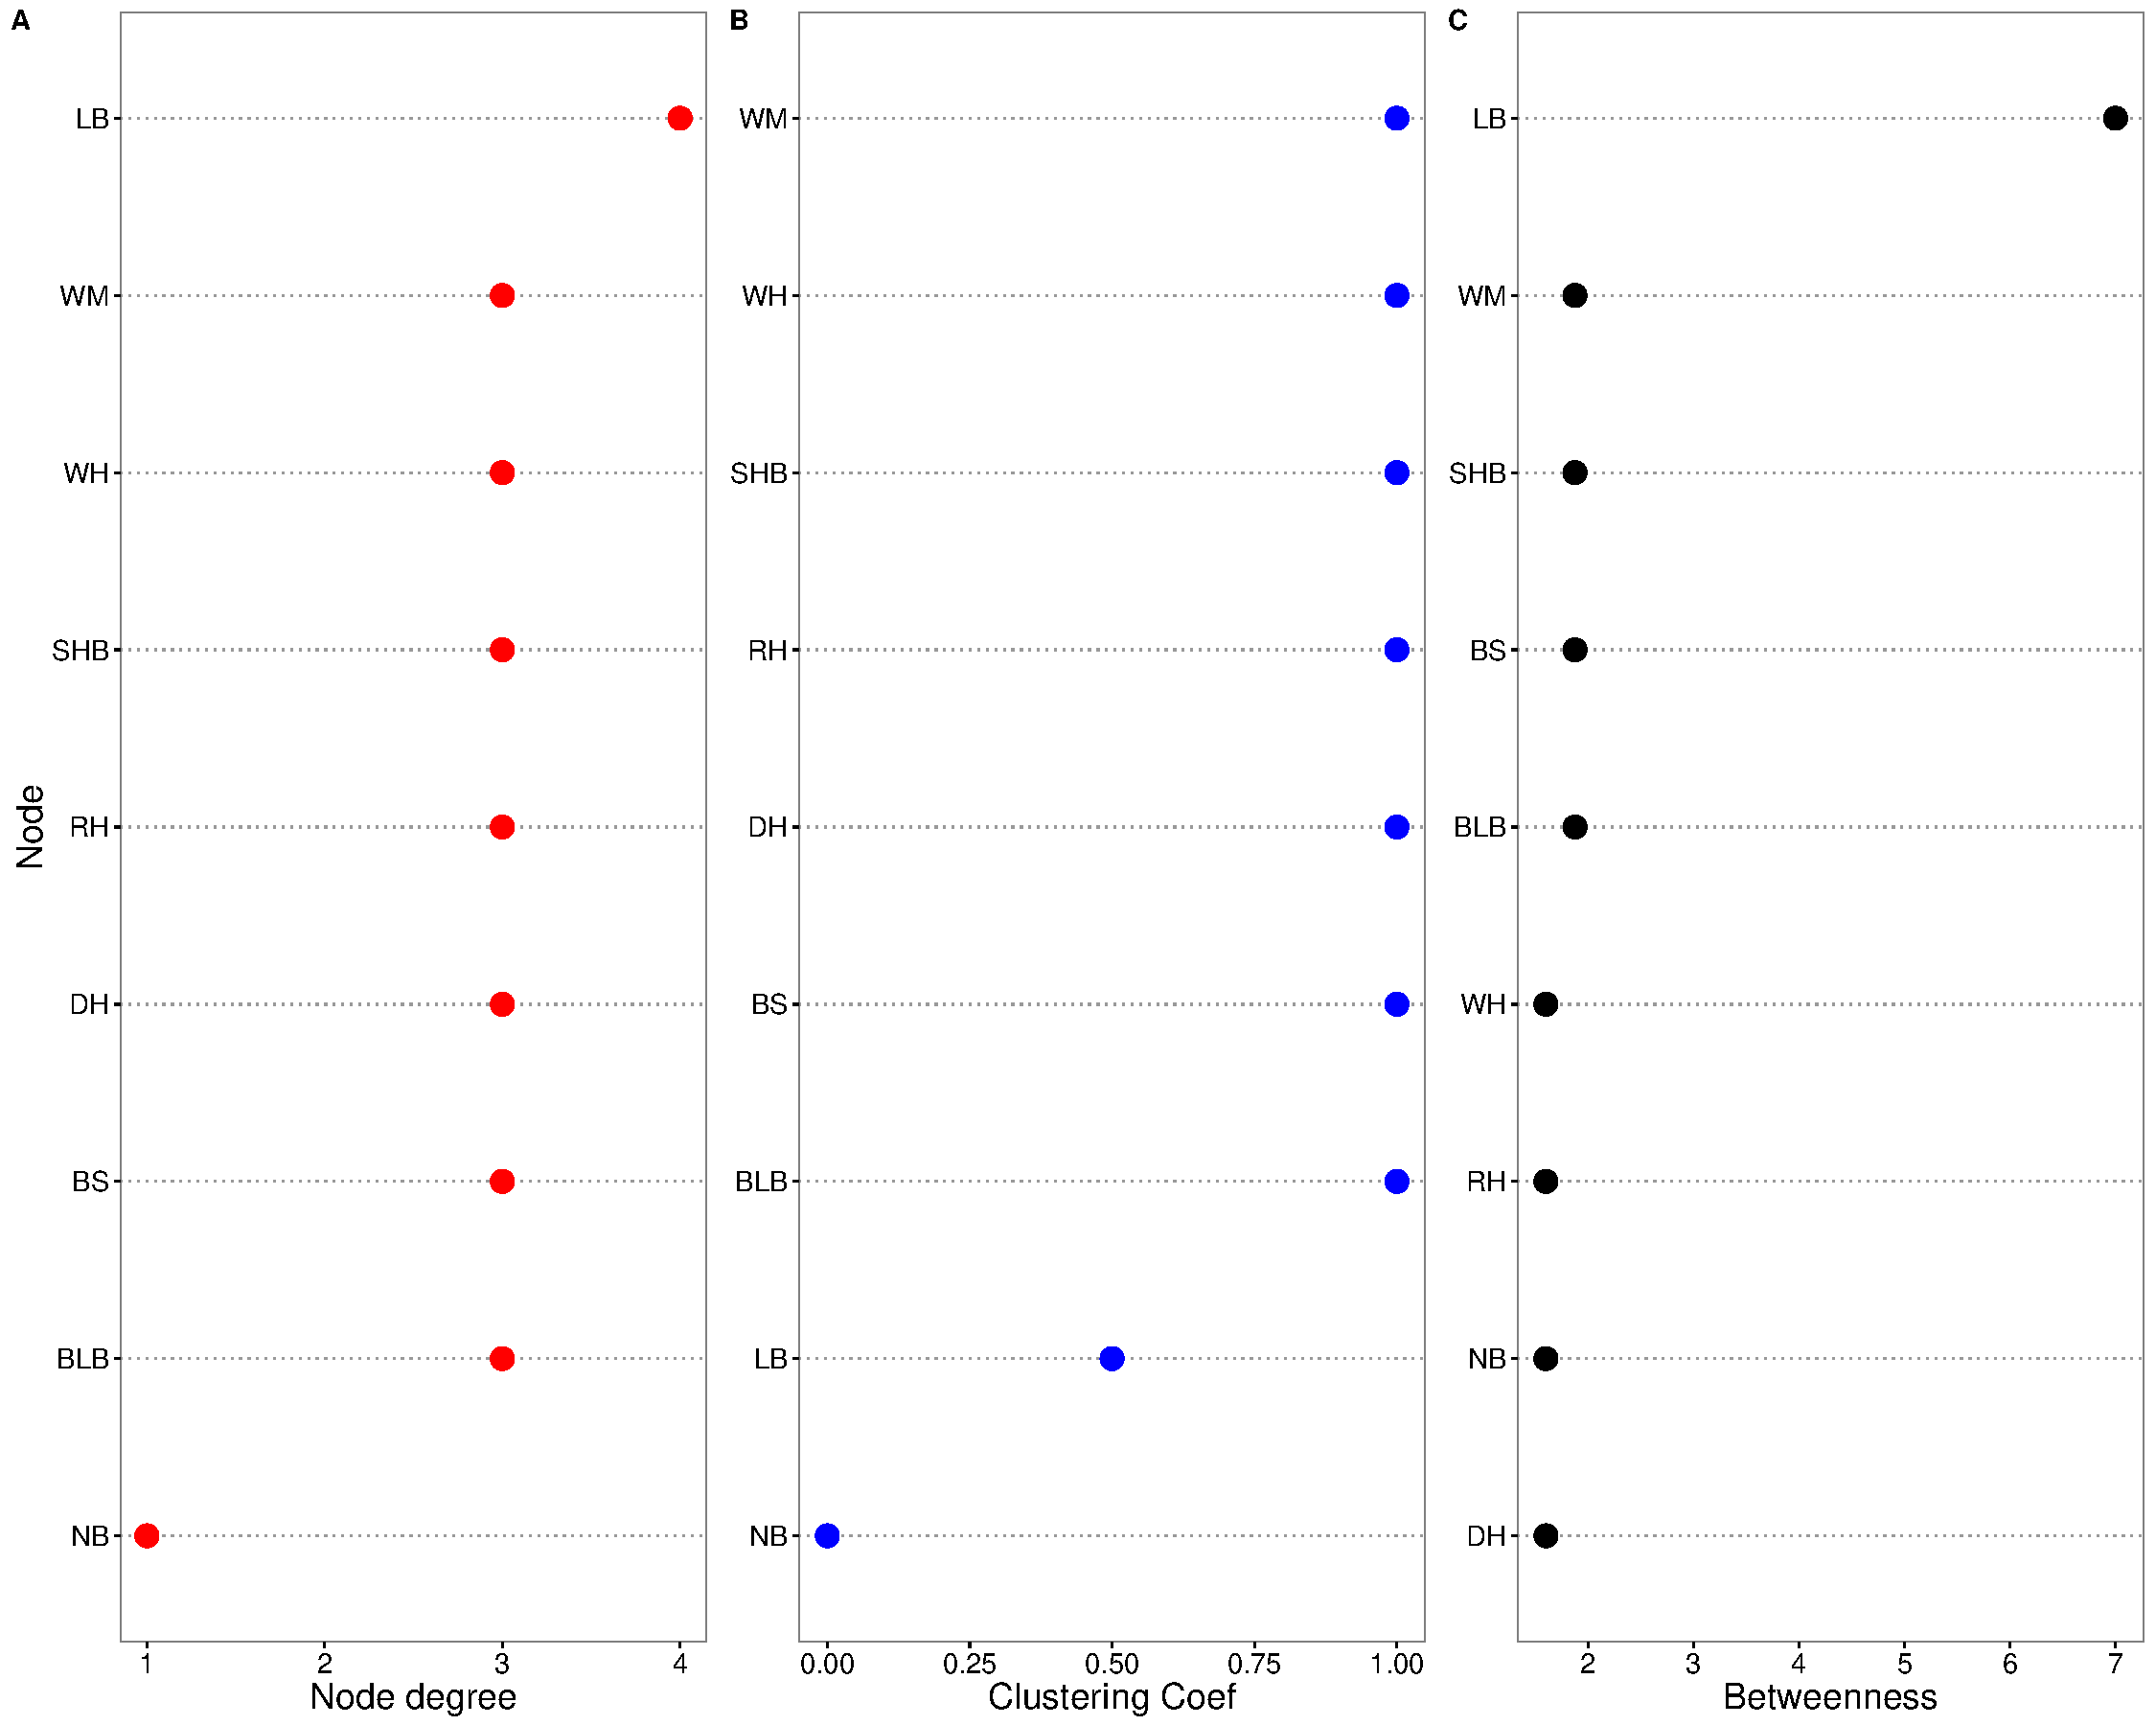
\includegraphics[width = 1\textwidth]{figures/nodepropOR_ds/nodepropOR_ds.pdf}
        \caption{Three centrality measures of the nodes in co-occurrence network of rice injuries in dry season at Odisha, India. A: node degree, B:clustering coefficient, and C:Betweenness, and.}
        \label{fig:nodepropCP_ds}
    \end{subfigure}
    \caption{Injuries in dry season at Odisha, India}
    \label{fig:OR_ds}
\end{figure}

\begin{figure}
    \centering
    \begin{subfigure}[b]{1\textwidth}
        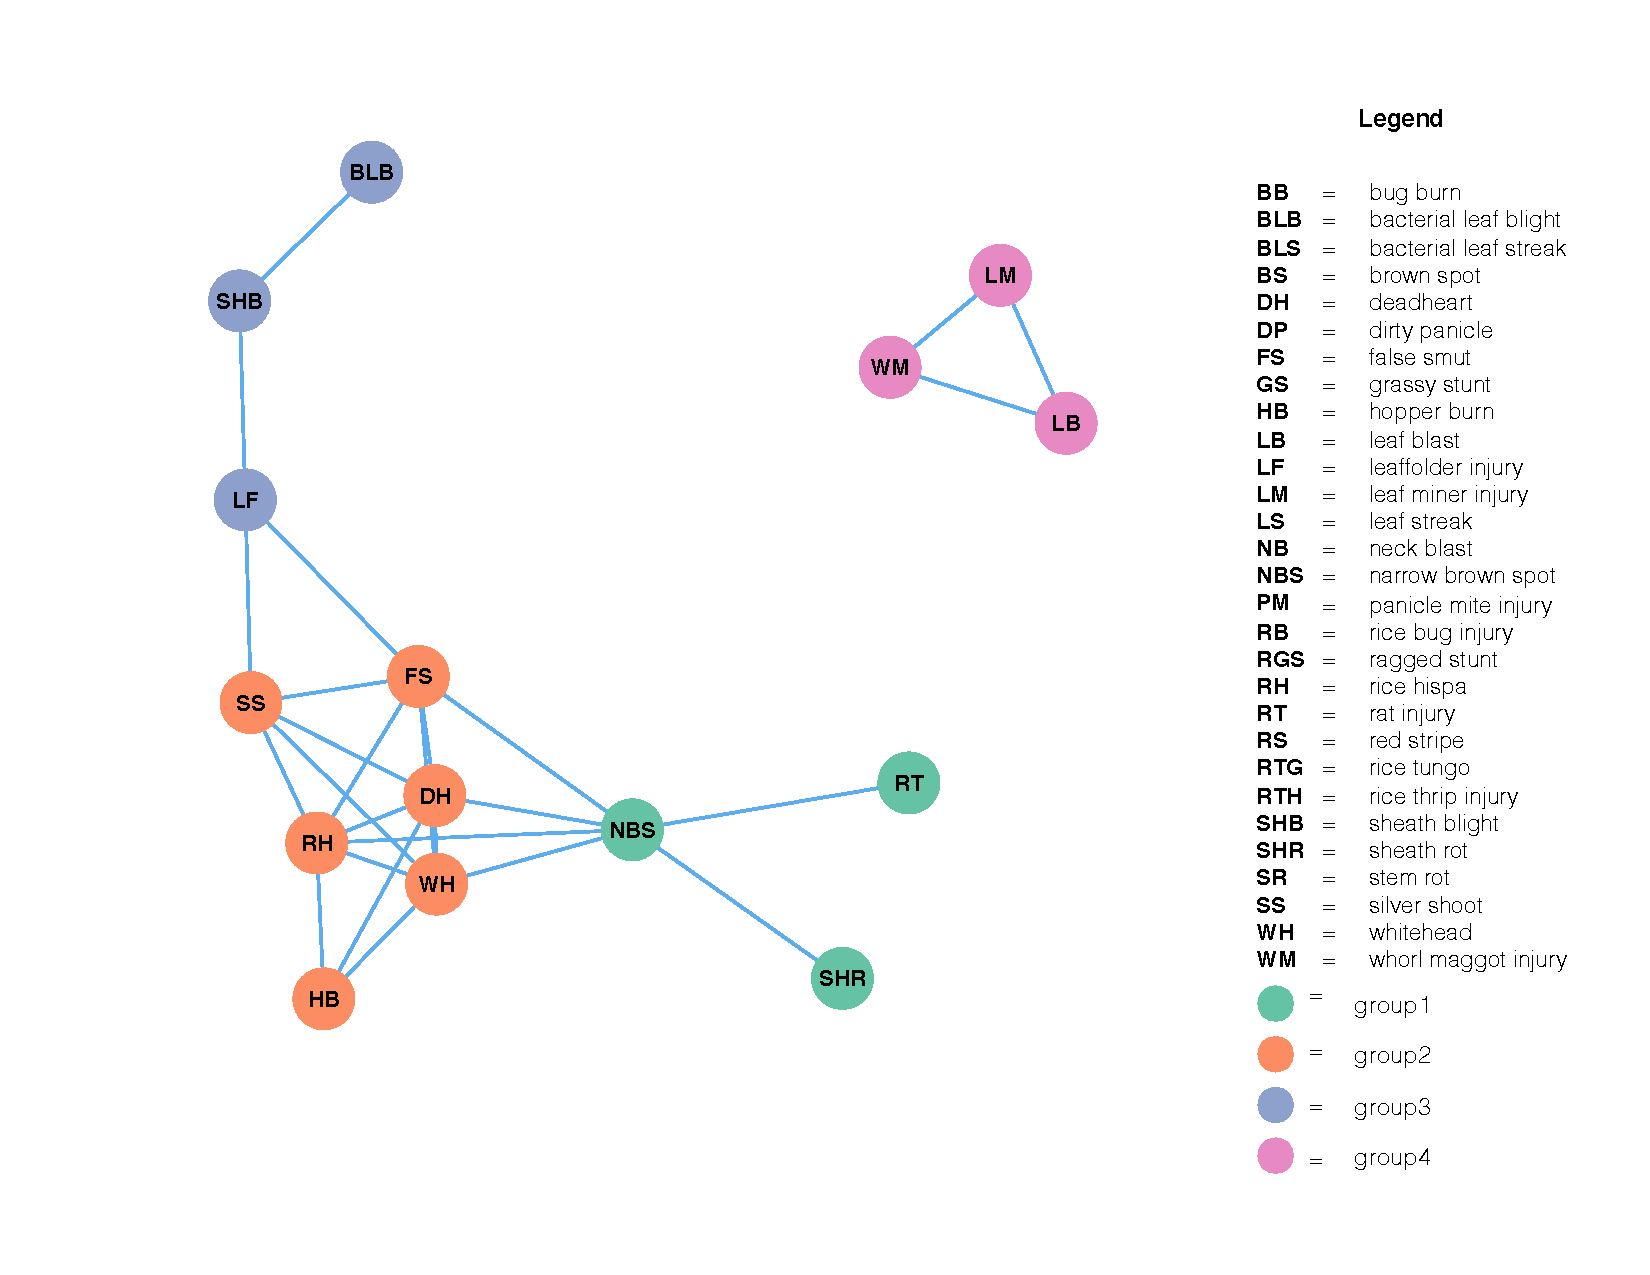
\includegraphics[width = 1\textwidth]{figures/networkOR_ws/networkOR_ws.pdf}
        \caption{Co-occurrence network of rice injuries in wet season at Odisha, India. The layout of the network graph is based on the Fruchterman-Reingold algorithm, which places nodes with stronger or more connections closer to each other.}
        \label{fig:gull}
    \end{subfigure}
    \begin{subfigure}[b]{1\textwidth}
        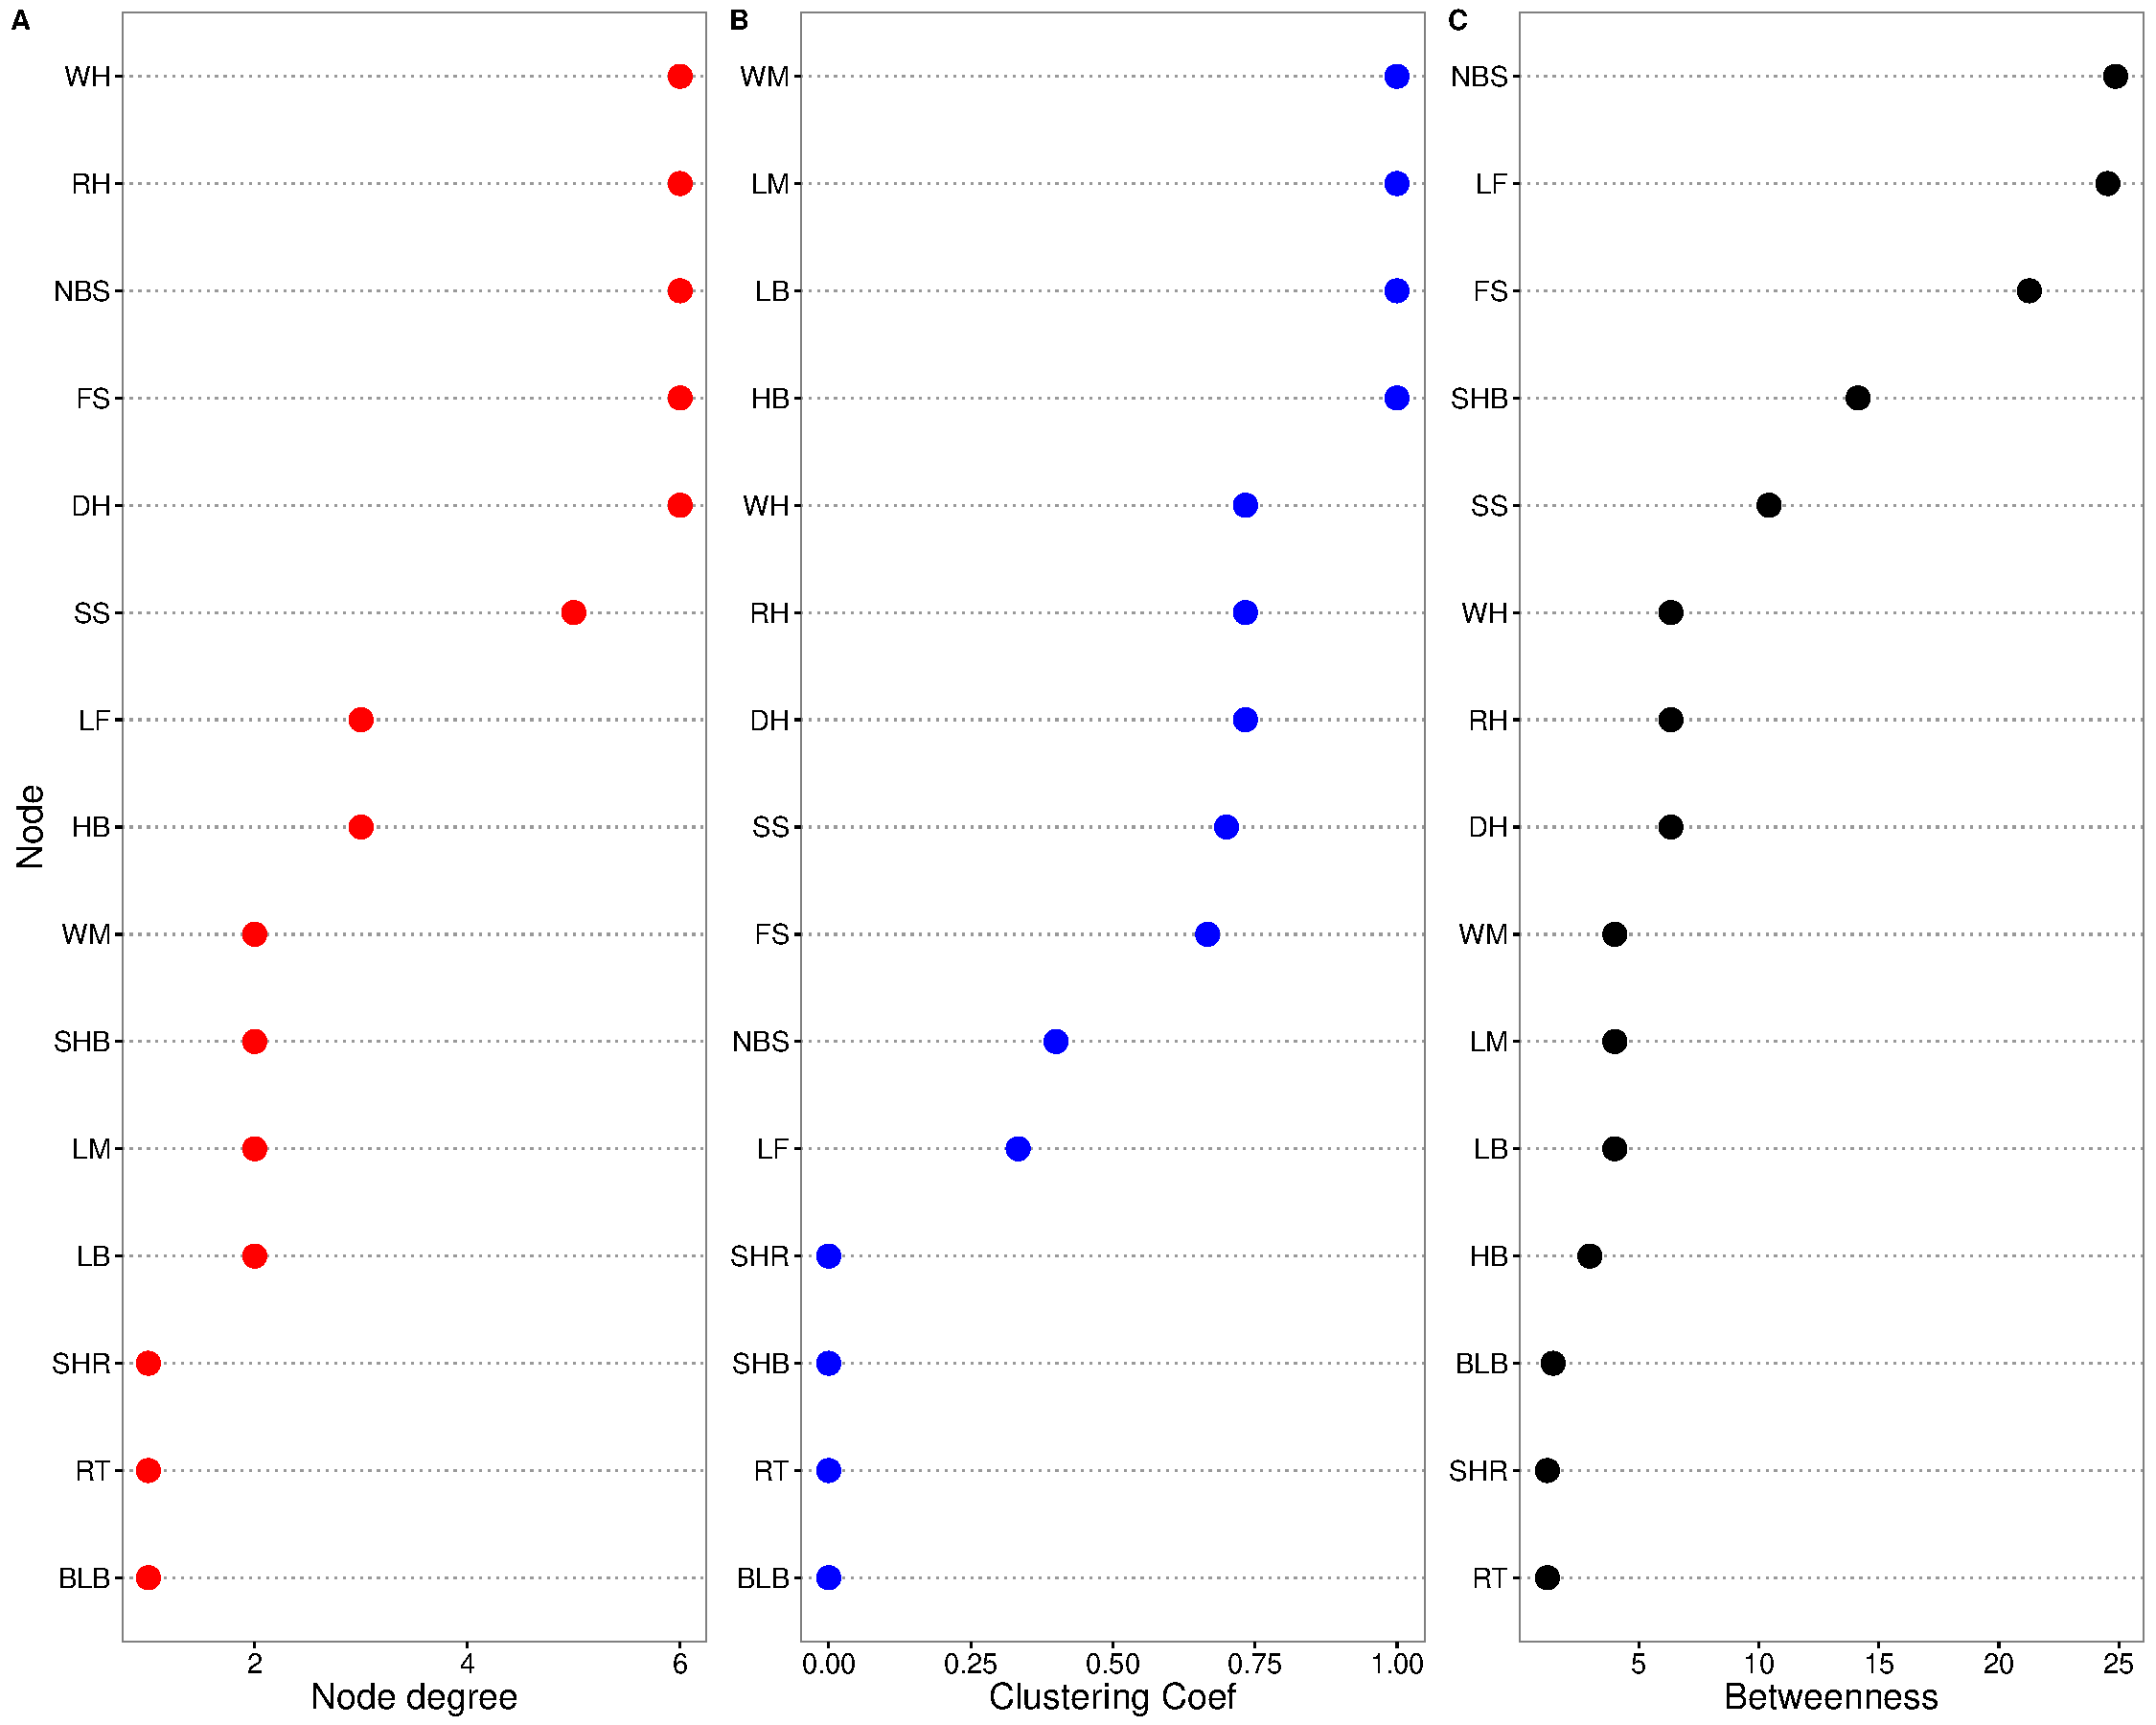
\includegraphics[width = 1\textwidth]{figures/nodepropOR_ws/nodepropOR_ws.pdf}
        \caption{Three centrality measures of the nodes in co-occurrence network of rice injuries in wet season at Odisha, India. A: node degree, B:clustering coefficient, and C:Betweenness, and.}
        \label{fig:nodepropCP_ds}
    \end{subfigure}
    \caption{Injuries in wer season at Odisha, India}
    \label{fig:OD_ws}
\end{figure}


\paragraph{Red River Delta, Vietnam}
 
Co-occurrence network of rice injuries in dry season (Fig. \ref{fig:networkRR_ds}) composed of ?? nodes and ?? associations. The network reveals three isolated groups, and two connected groups of injury profiles. Group1 and group3 were linked with BB. Group3 was the biggest among the others. In this group, SHB, BS were nodes showing high centrality (table \ref{table:nodepropRR_ds}). If they were observed in rice fields, there was high chance to observe other injuries of group3 in the fields too.

Wet season network (Fig. \ref{fig:networkRR_ws})) composed of ?? injuries with ?? associations. It reveals 4 connected groups and one isolated small group of injury profiles. Group4 was located that could connect to Group2, 3, 5. According to table\ref{table:nodepropRR_ws}, BLB, DP could be a good indicator, because it was likely to occur (high betweenness) and when it presented, other injuries in other group, except group5 (high node degree). 


\begin{figure}
    \centering
    \begin{subfigure}[b]{1\textwidth}
        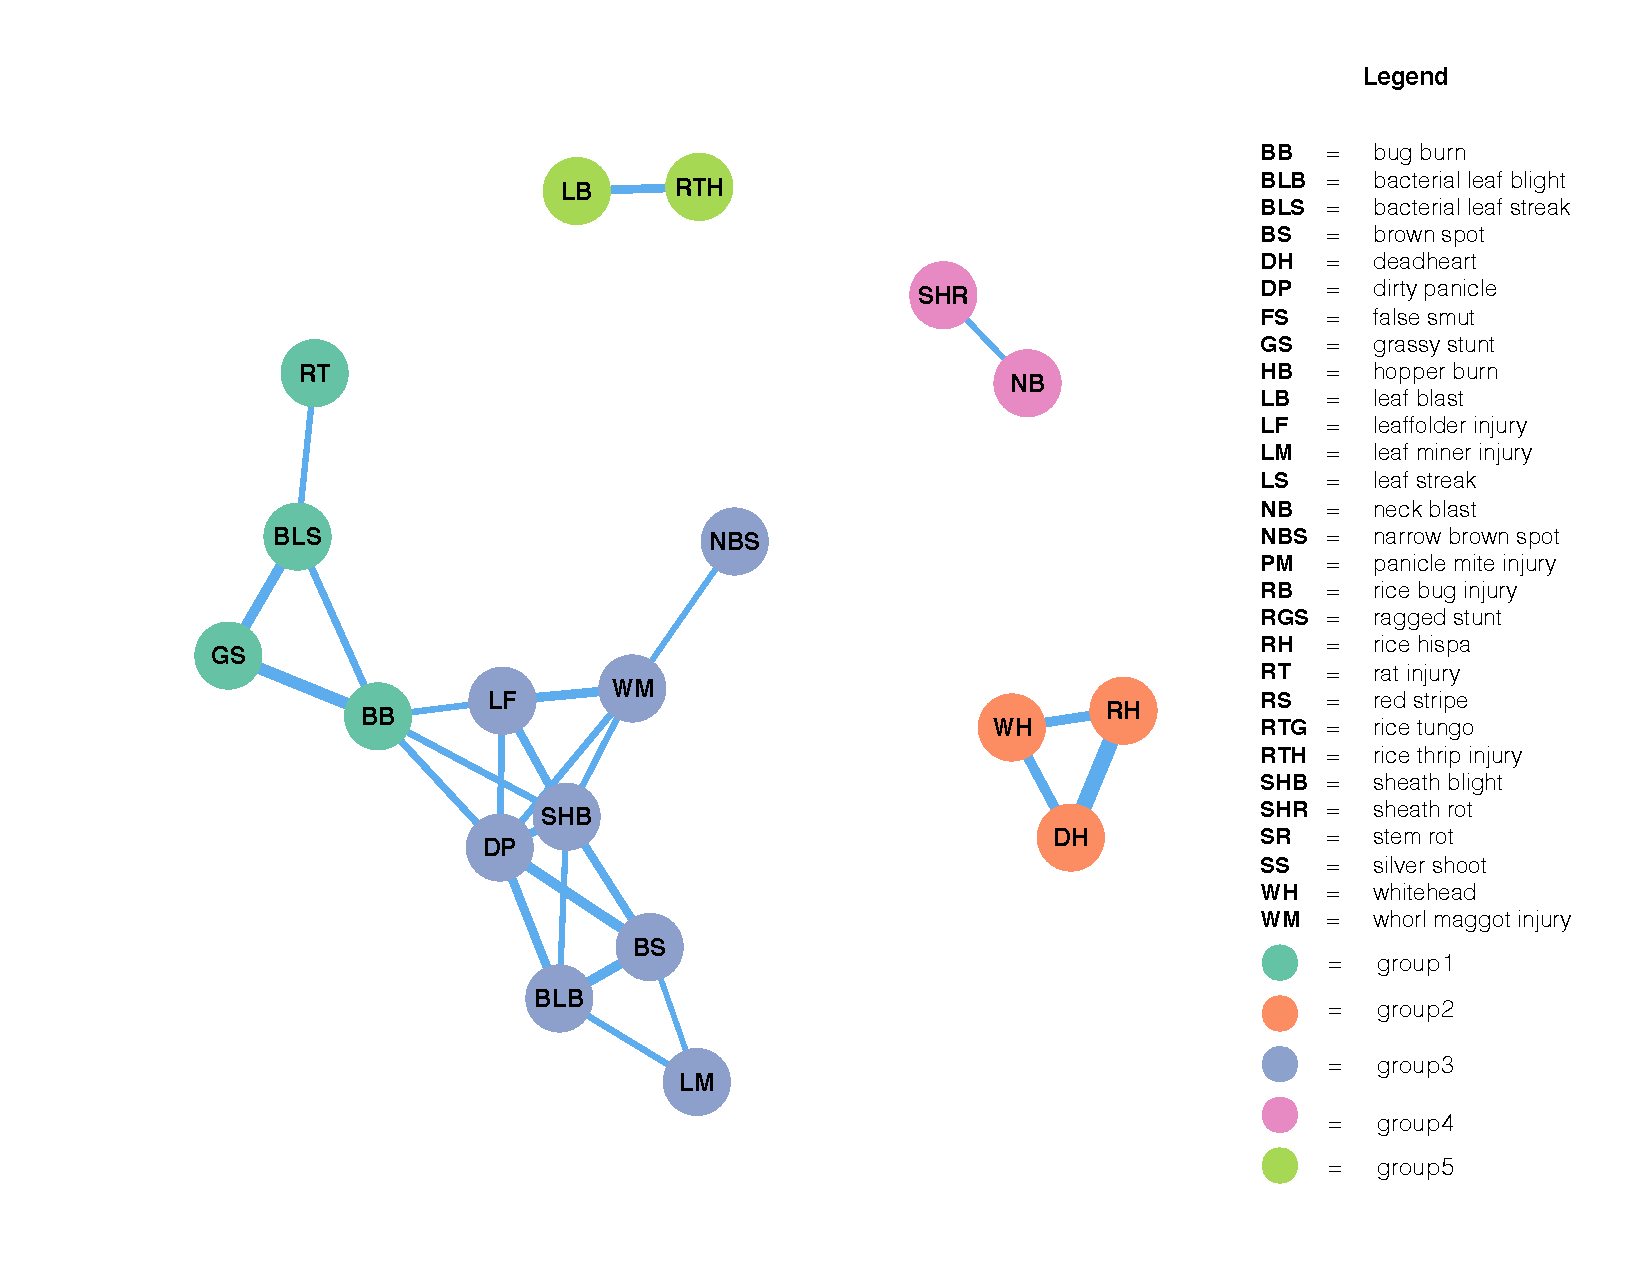
\includegraphics[width = 1\textwidth]{figures/networkRR_ds/networkRR_ds.pdf}
        \caption{Co-occurrence network of rice injuries in dry season at Red River Delta, Vietnam. The layout of the network graph is based on the Fruchterman-Reingold algorithm, which places nodes with stronger or more connections closer to each other.}
        \label{fig:gull}
    \end{subfigure}
    \begin{subfigure}[b]{1\textwidth}
        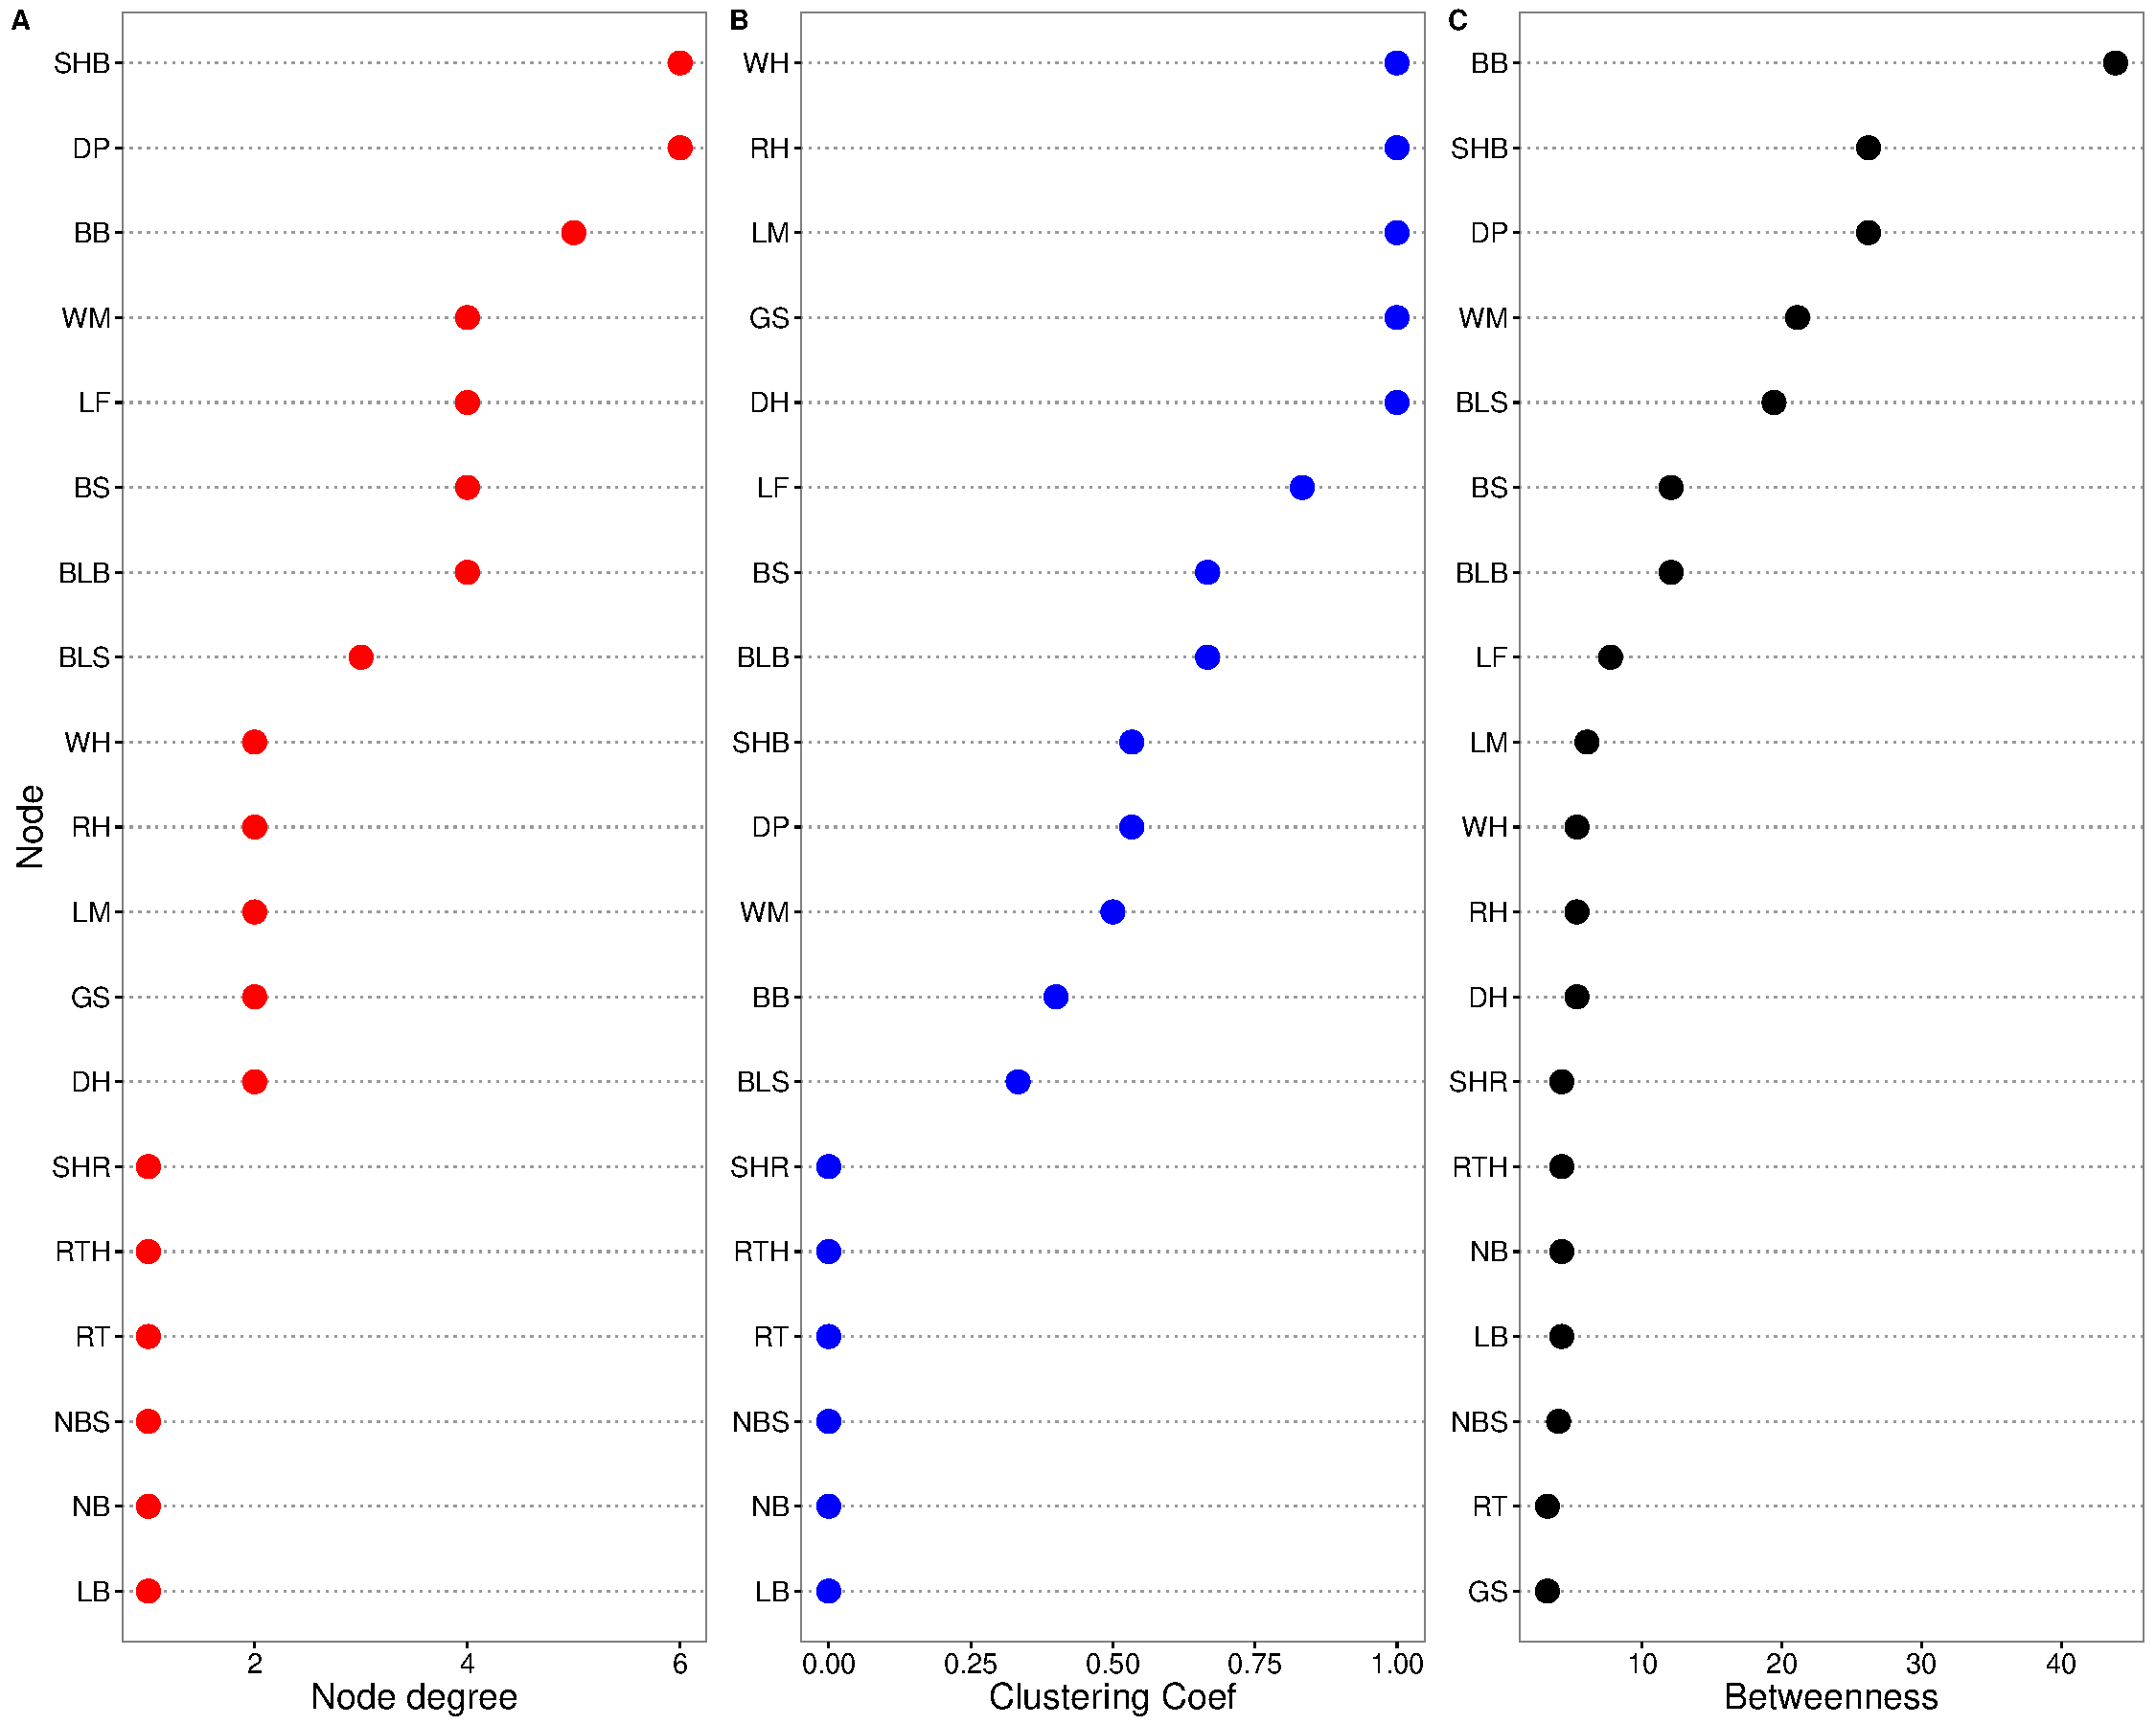
\includegraphics[width = 1\textwidth]{figures/nodepropRR_ds/nodepropRR_ds.pdf}
        \caption{Three centrality measures of the nodes in co-occurrence network of rice injuries in dry season at Red River Delta, Vietnam. A: node degree, B:clustering coefficient, and C:Betweenness}
        \label{fig:nodepropCP_ds}
    \end{subfigure}
    \caption{Pictures of animals}
    \label{fig:animals}
\end{figure}

\begin{figure}
    \centering
    \begin{subfigure}[b]{1\textwidth}
        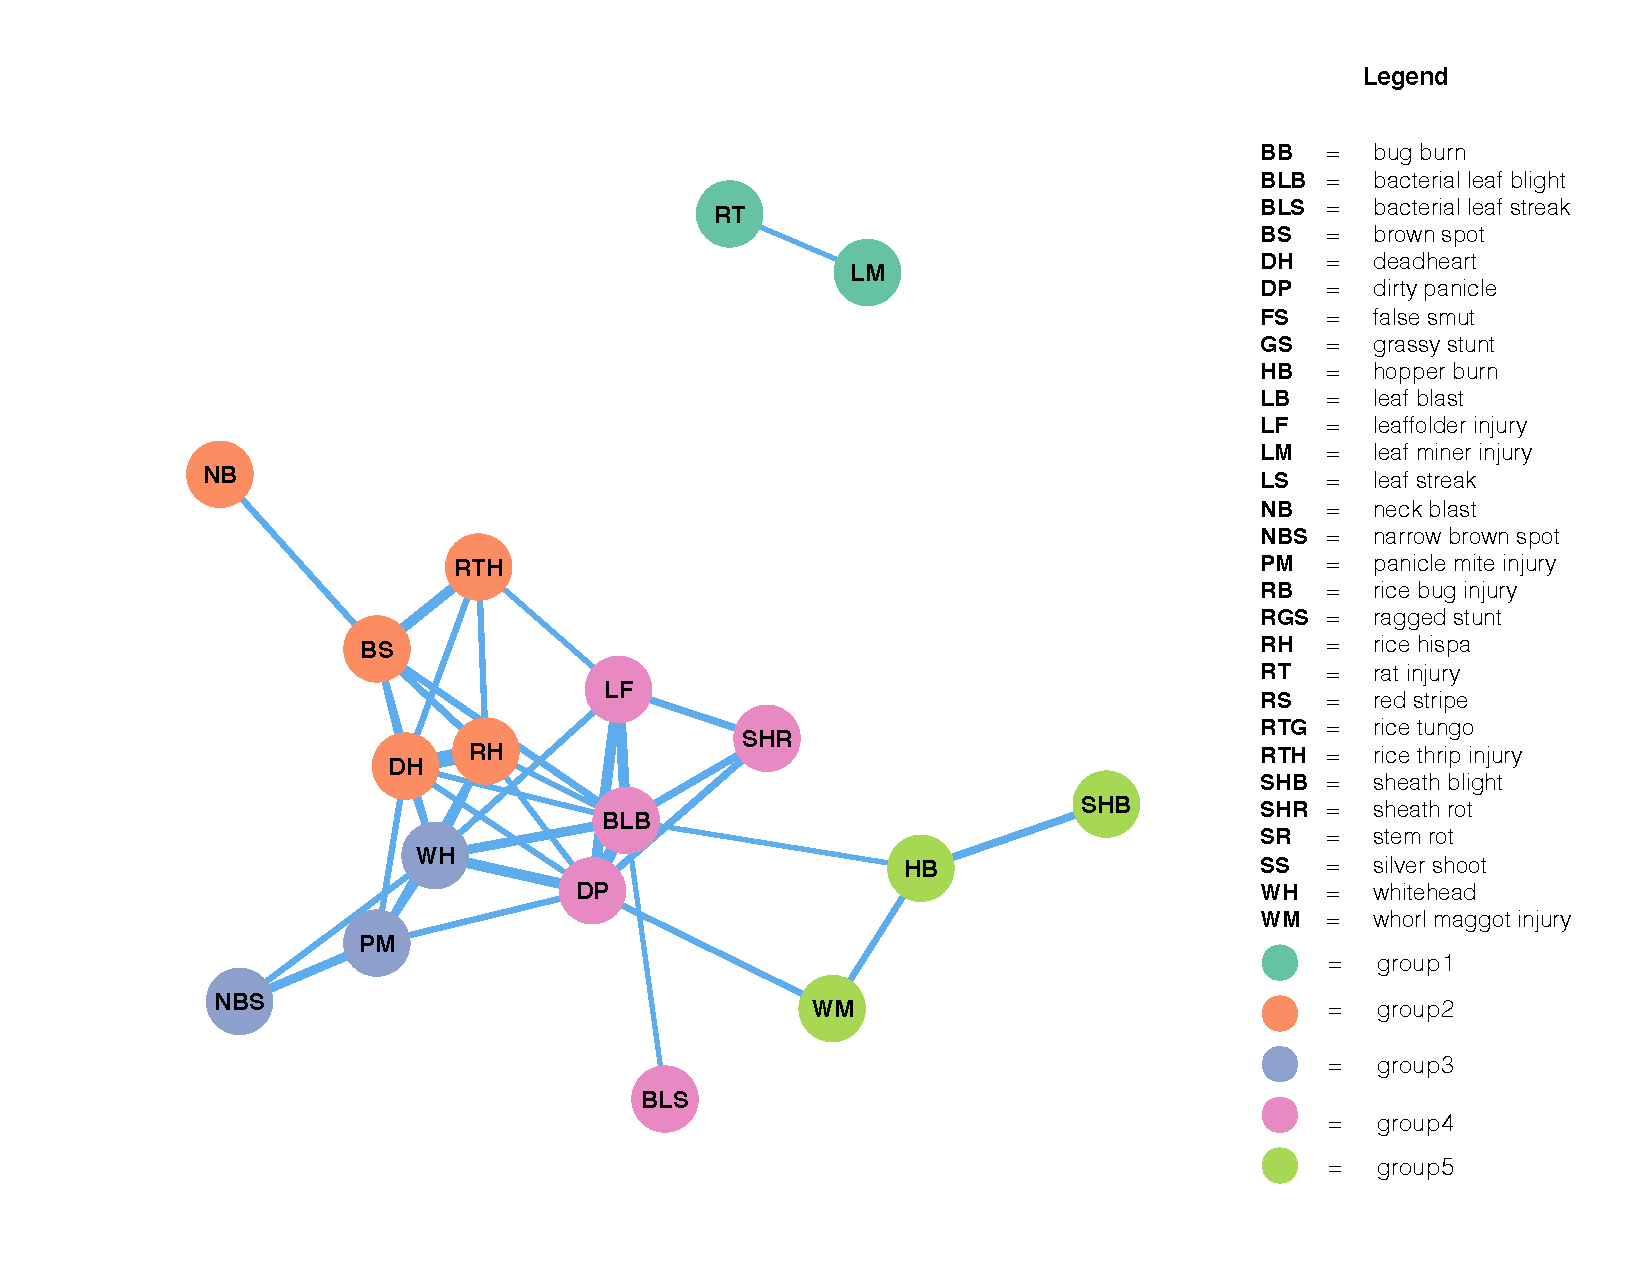
\includegraphics[width = 1\textwidth]{figures/networkRR_ws/networkRR_ws.pdf}
        \caption{Co-occurrence network of rice injuries in wet season at Red River Delta, Vietnam. The layout of the network graph is based on the Fruchterman-Reingold algorithm, which places nodes with stronger or more connections closer to each other.}
        \label{fig:gull}
    \end{subfigure}
    \begin{subfigure}[b]{1\textwidth}
        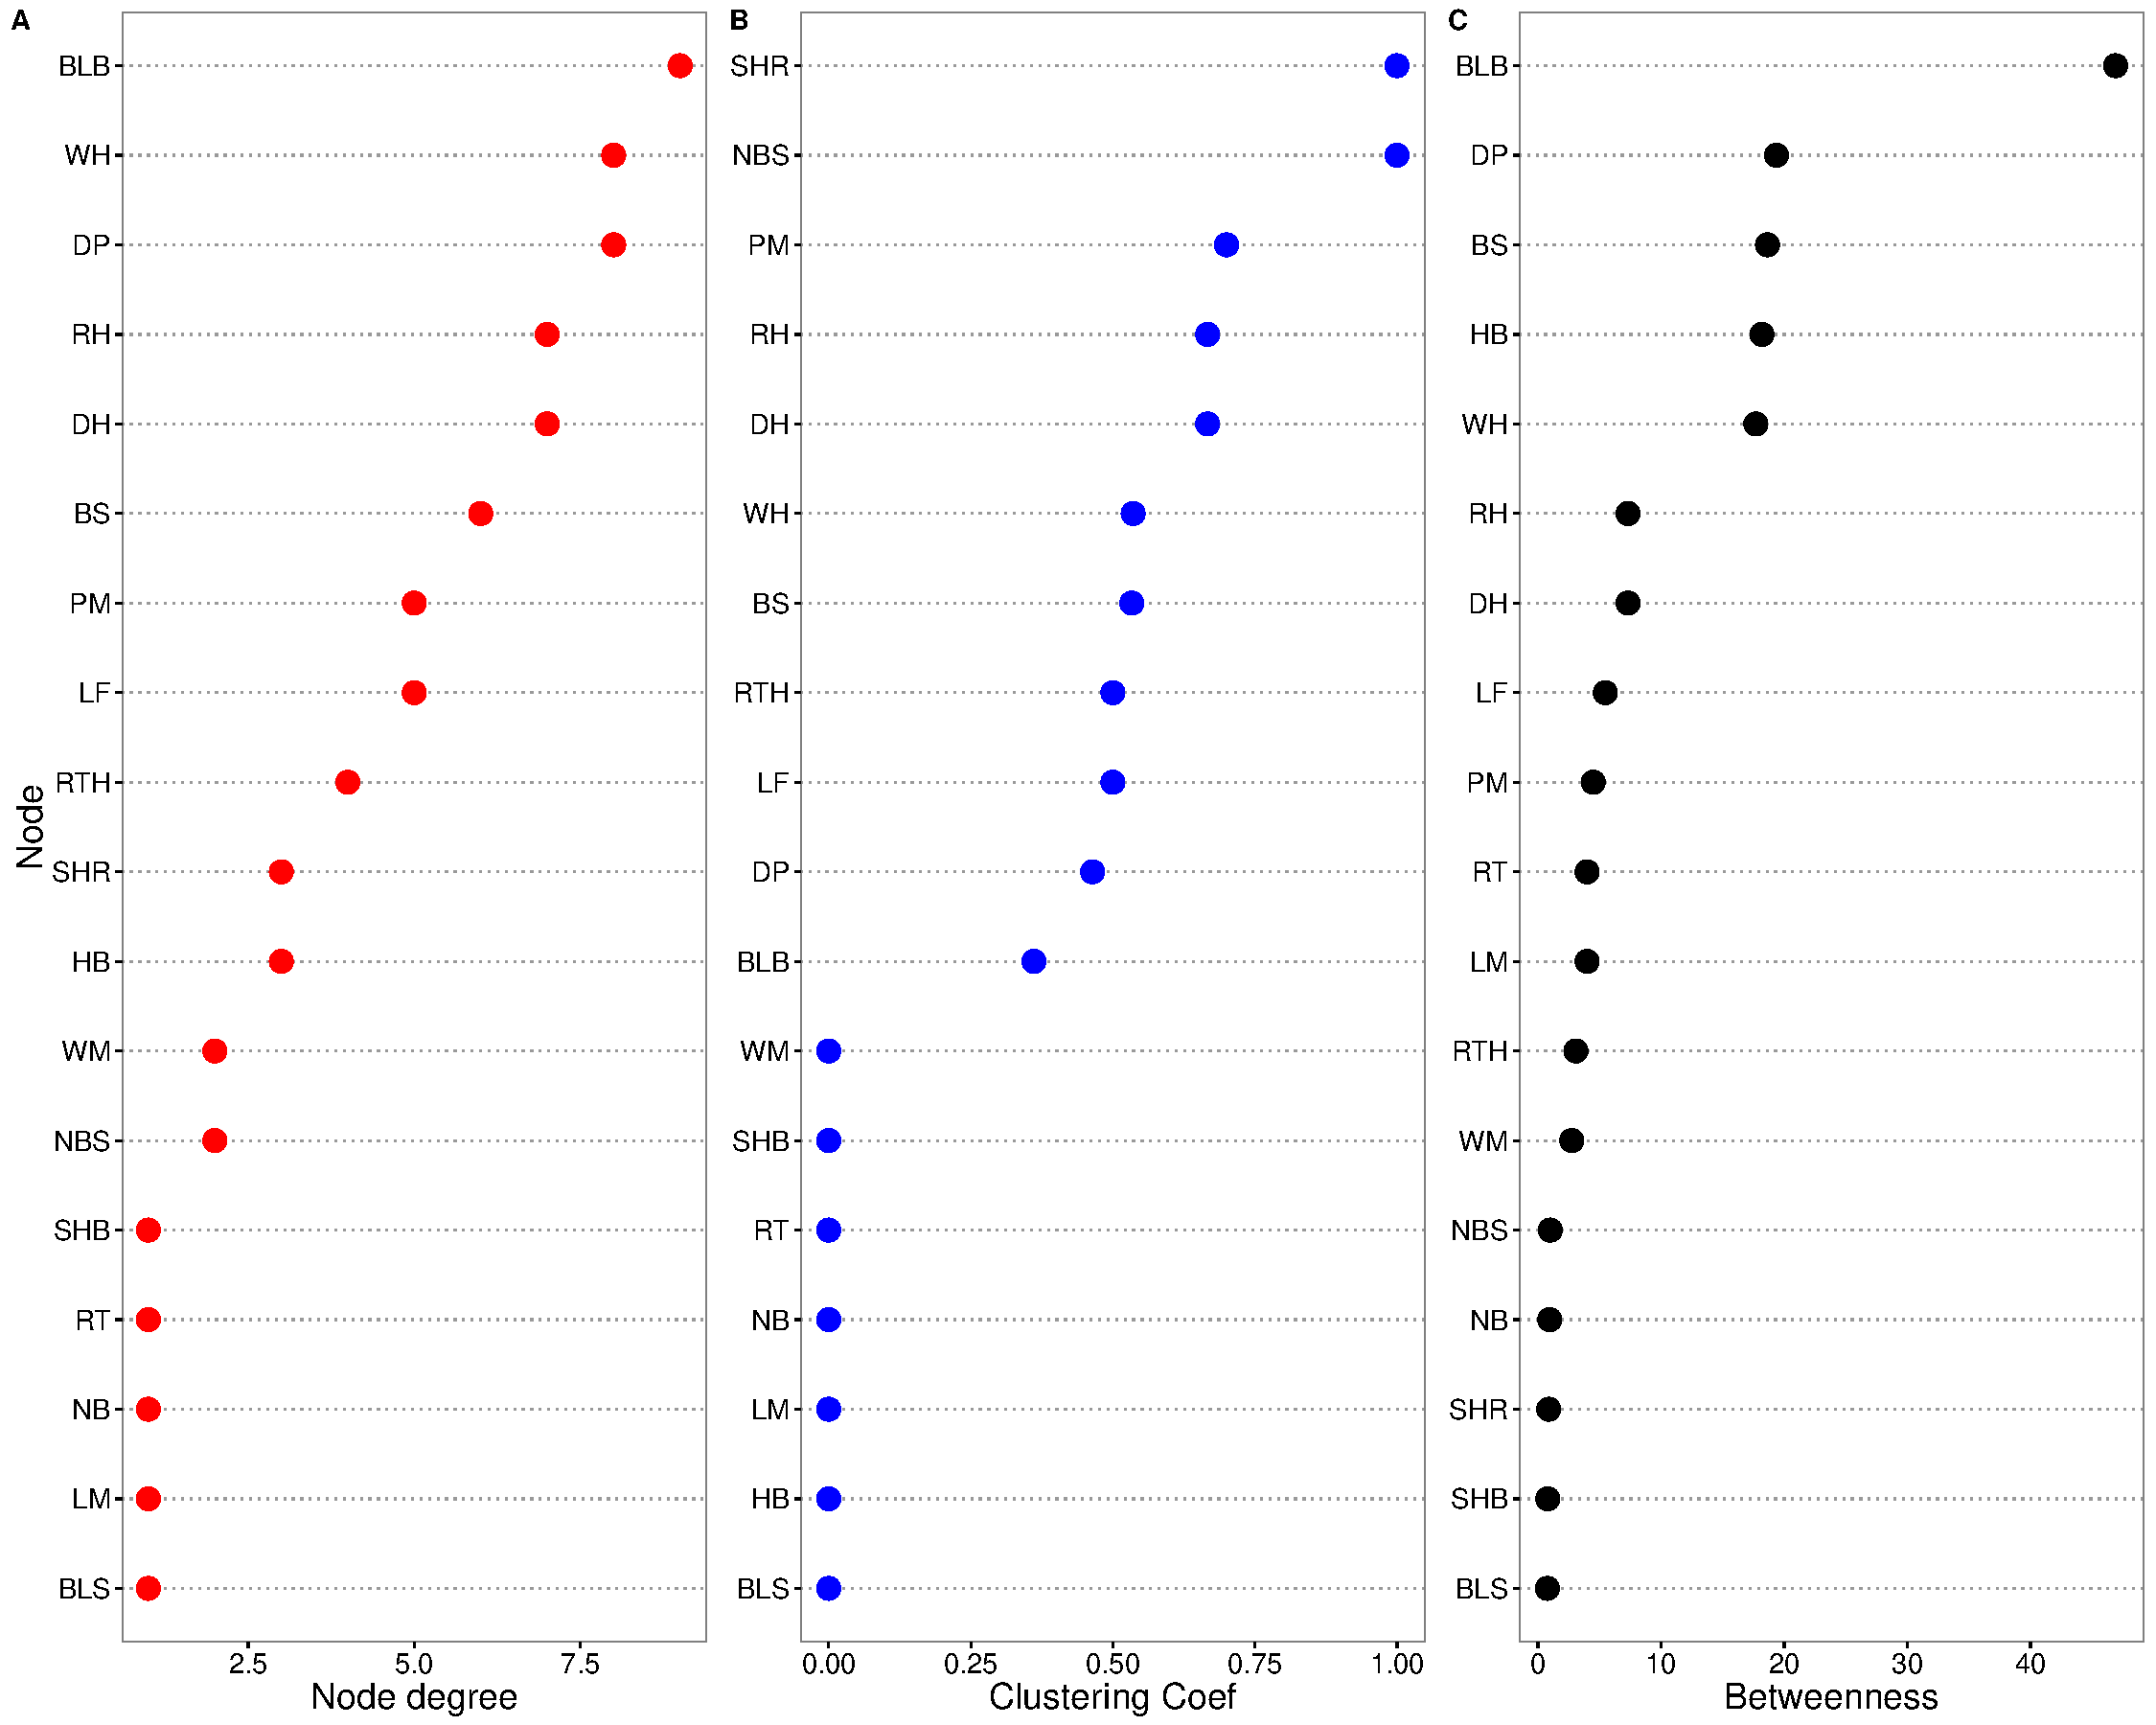
\includegraphics[width = 1\textwidth]{figures/nodepropRR_ws/nodepropRR_ws.pdf}
        \caption{Three centrality measures of the nodes in co-occurrence network of rice injuries in wet season at Red River Delta, Vietnam. A: node degree, B:clustering coefficient, and C:Betweenness}
        \label{fig:nodepropCP_ds}
    \end{subfigure}
    \caption{Rice injuries in wet season in Red River Delta, Vietnam}
    \label{fig:animals}
\end{figure}


\paragraph{Tamil Nadu, India}

The dry season network (Fig \ref{fig:networkTM_ds}) revealed three clustered groups of injury profiles. One of them was separated from other two. Group1 was condensed, which differ from group2 that injuries were placed further. SHB and BLB were disconnected to the rest.  BS and WH highly tended to occur in this season (high betweenness).  Because clustering coefficient value of members in group2 less than group1, injuries in group2 might occur together with one or two more injuries. But in group1, the combination was more complex than.

Figure \ref{fig:networkTM_ws} presented co-occurrence network of injury profiles in dry season. Network resulted three groups of injury profiles. Compared to other groups, group3 had less connection. Group1 had high node degree injuires.


\begin{figure}
    \centering
    \begin{subfigure}[b]{1\textwidth}
        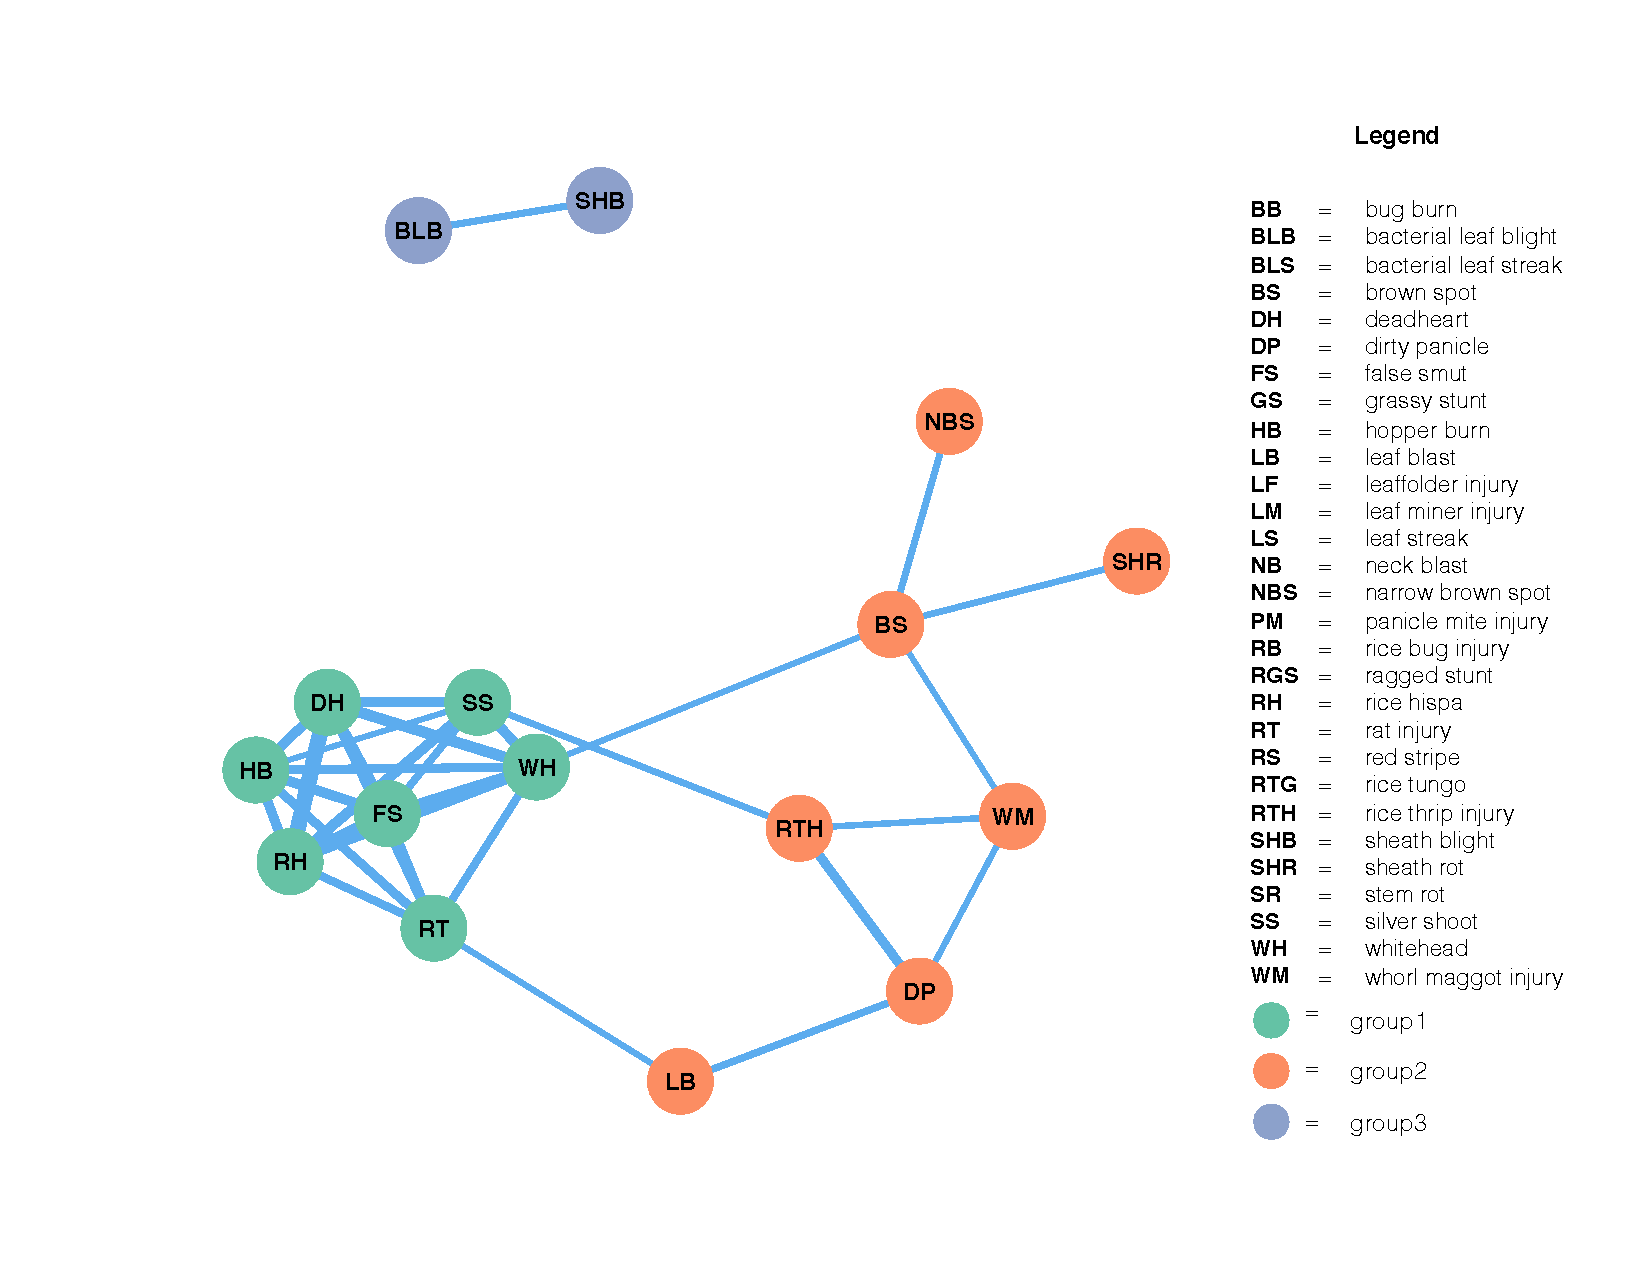
\includegraphics[width = 1\textwidth]{figures/networkTM_ds/networkTM_ds.pdf}
        \caption{Co-occurrence network of rice injuries in dry season at Tamil Nadu, India. The layout of the network graph is based on the Fruchterman-Reingold algorithm, which places nodes with stronger or more connections closer to each other.}
        \label{fig:networkTM_ds}
    \end{subfigure}
    \begin{subfigure}[b]{1\textwidth}
        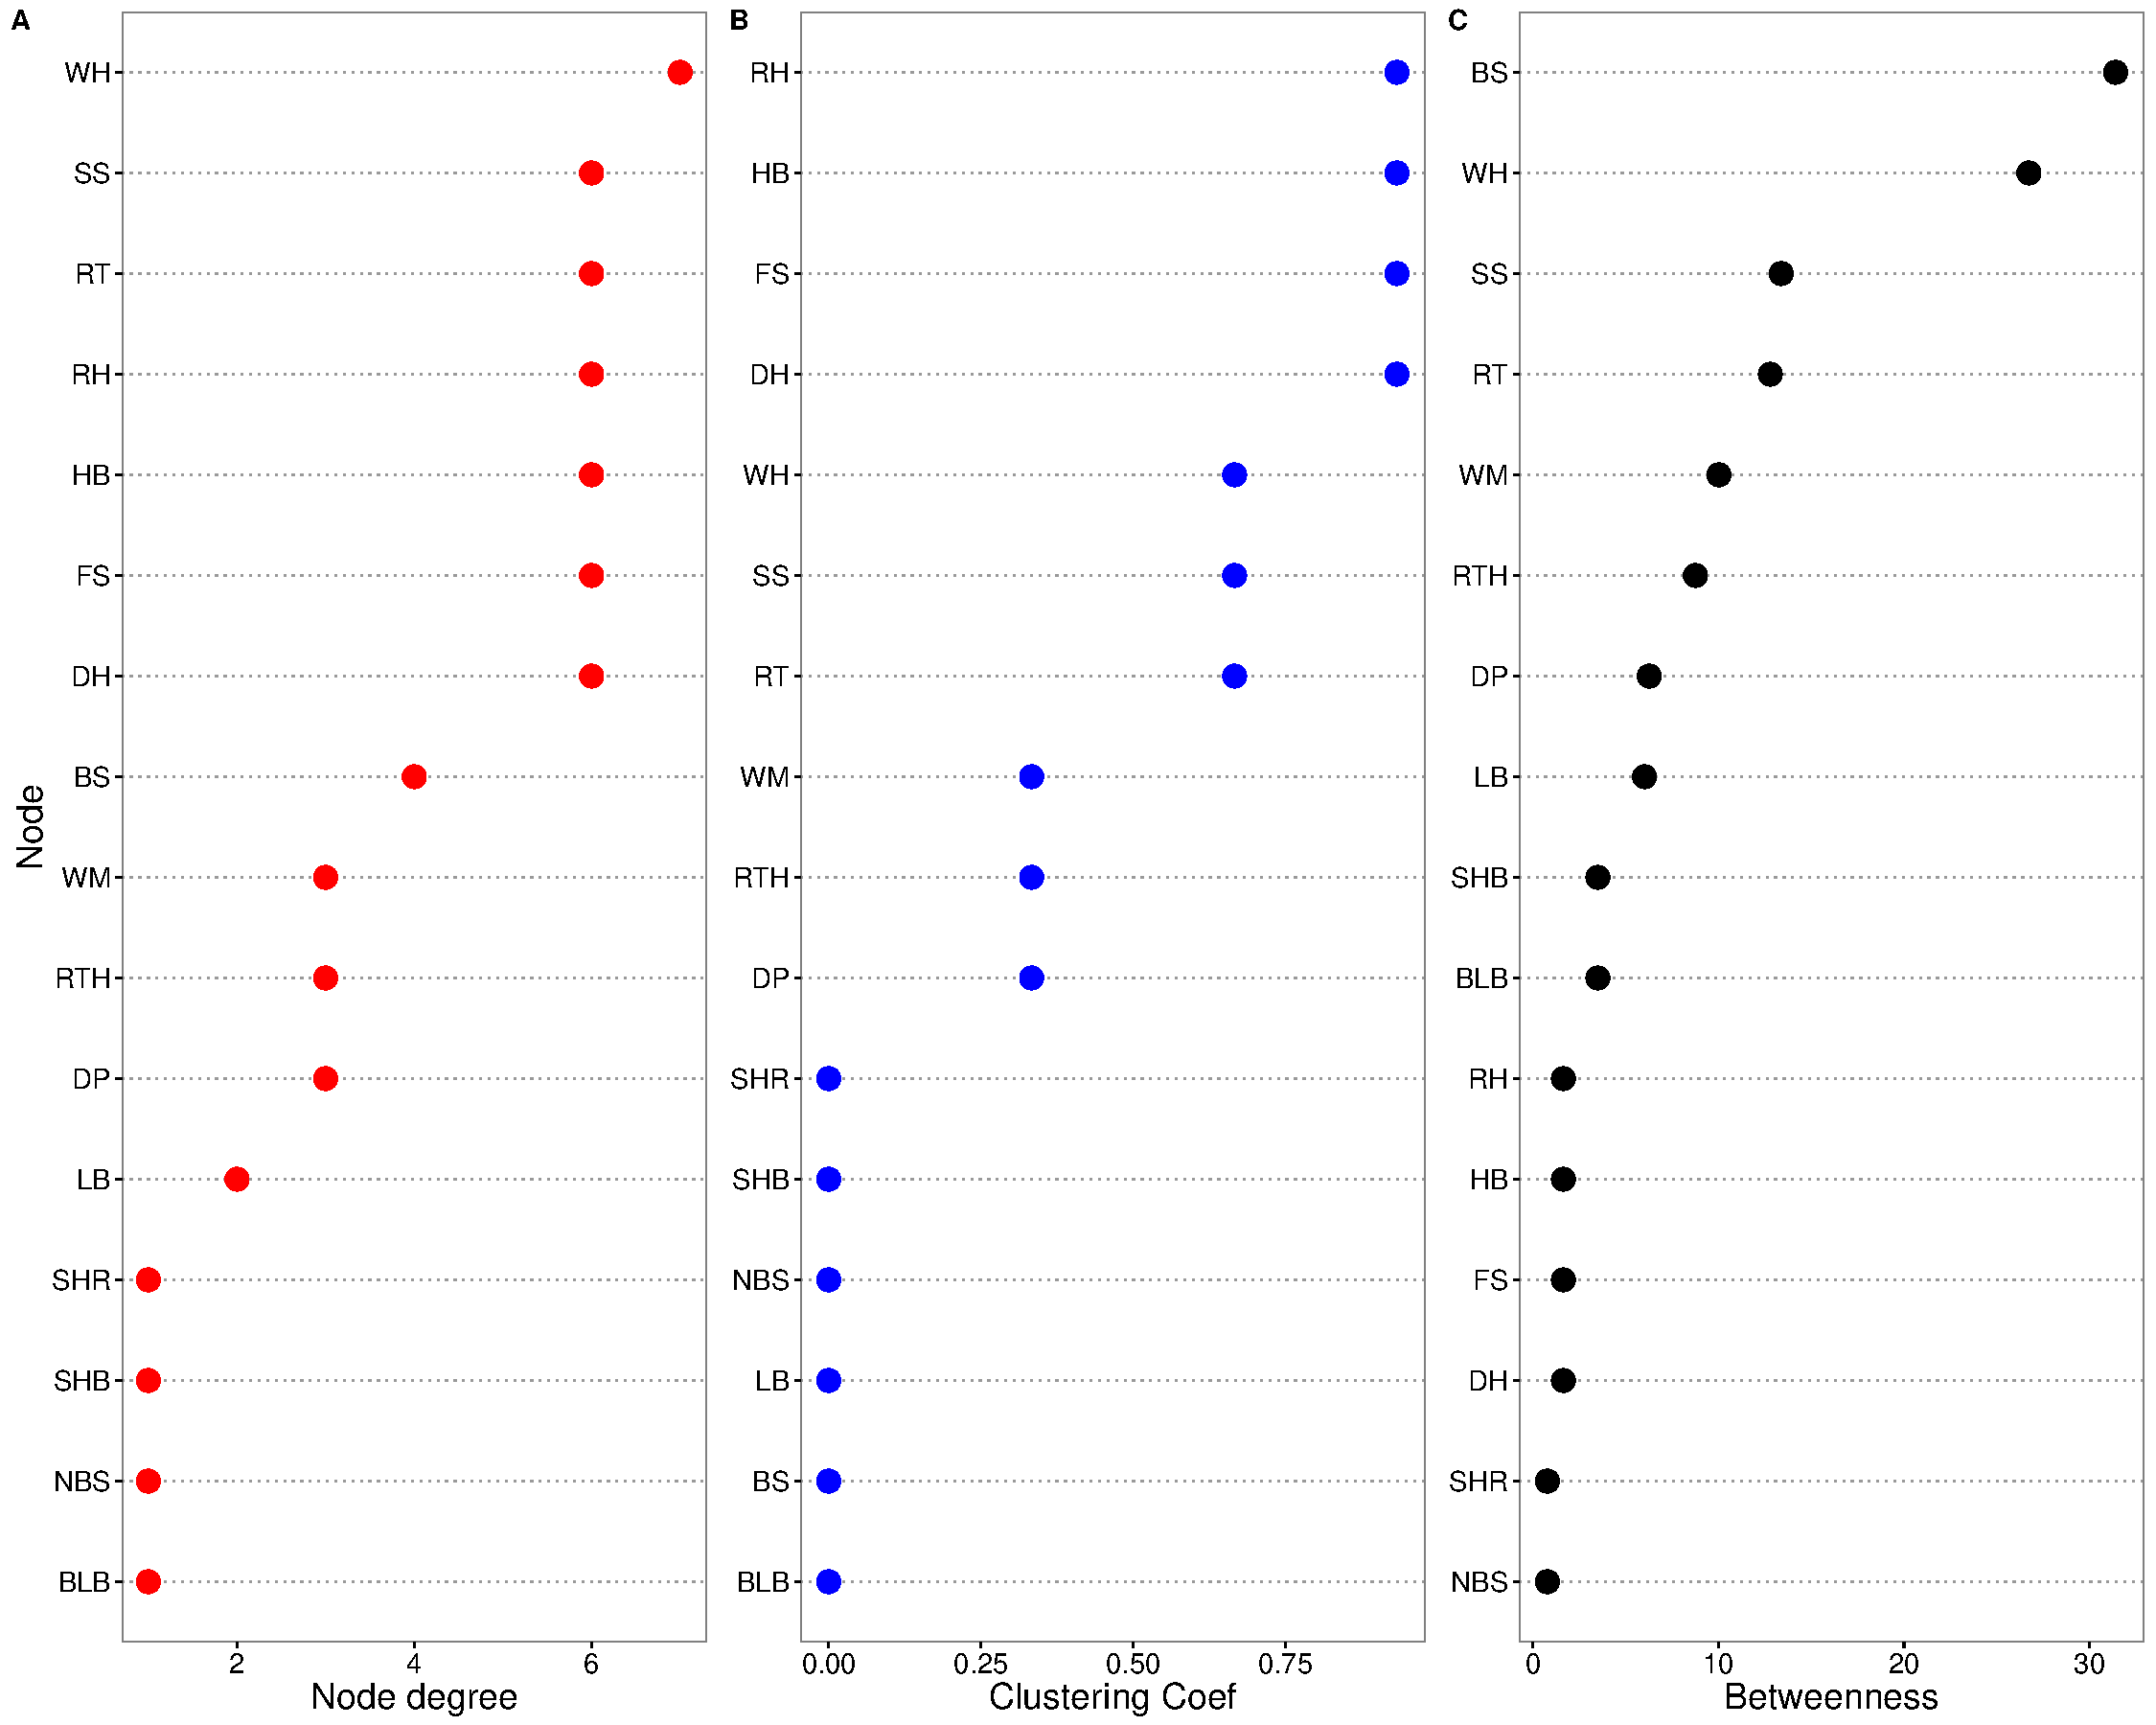
\includegraphics[width = 1\textwidth]{figures/nodepropTM_ds/nodepropTM_ds.pdf}
        \caption{Three centrality measures of the nodes in co-occurrence network of rice injuries in dry season at Tamil Nadu, India. A: node degree, B:clustering coefficient, and C:Betweenness, and.}
        \label{fig:nodepropTM_ds}
    \end{subfigure}
    \caption{Rice injuries in dry season in Tamil Nadu, India}
    \label{fig:TM_ds}
\end{figure}

\begin{figure}
    \centering
    \begin{subfigure}[b]{1\textwidth}
        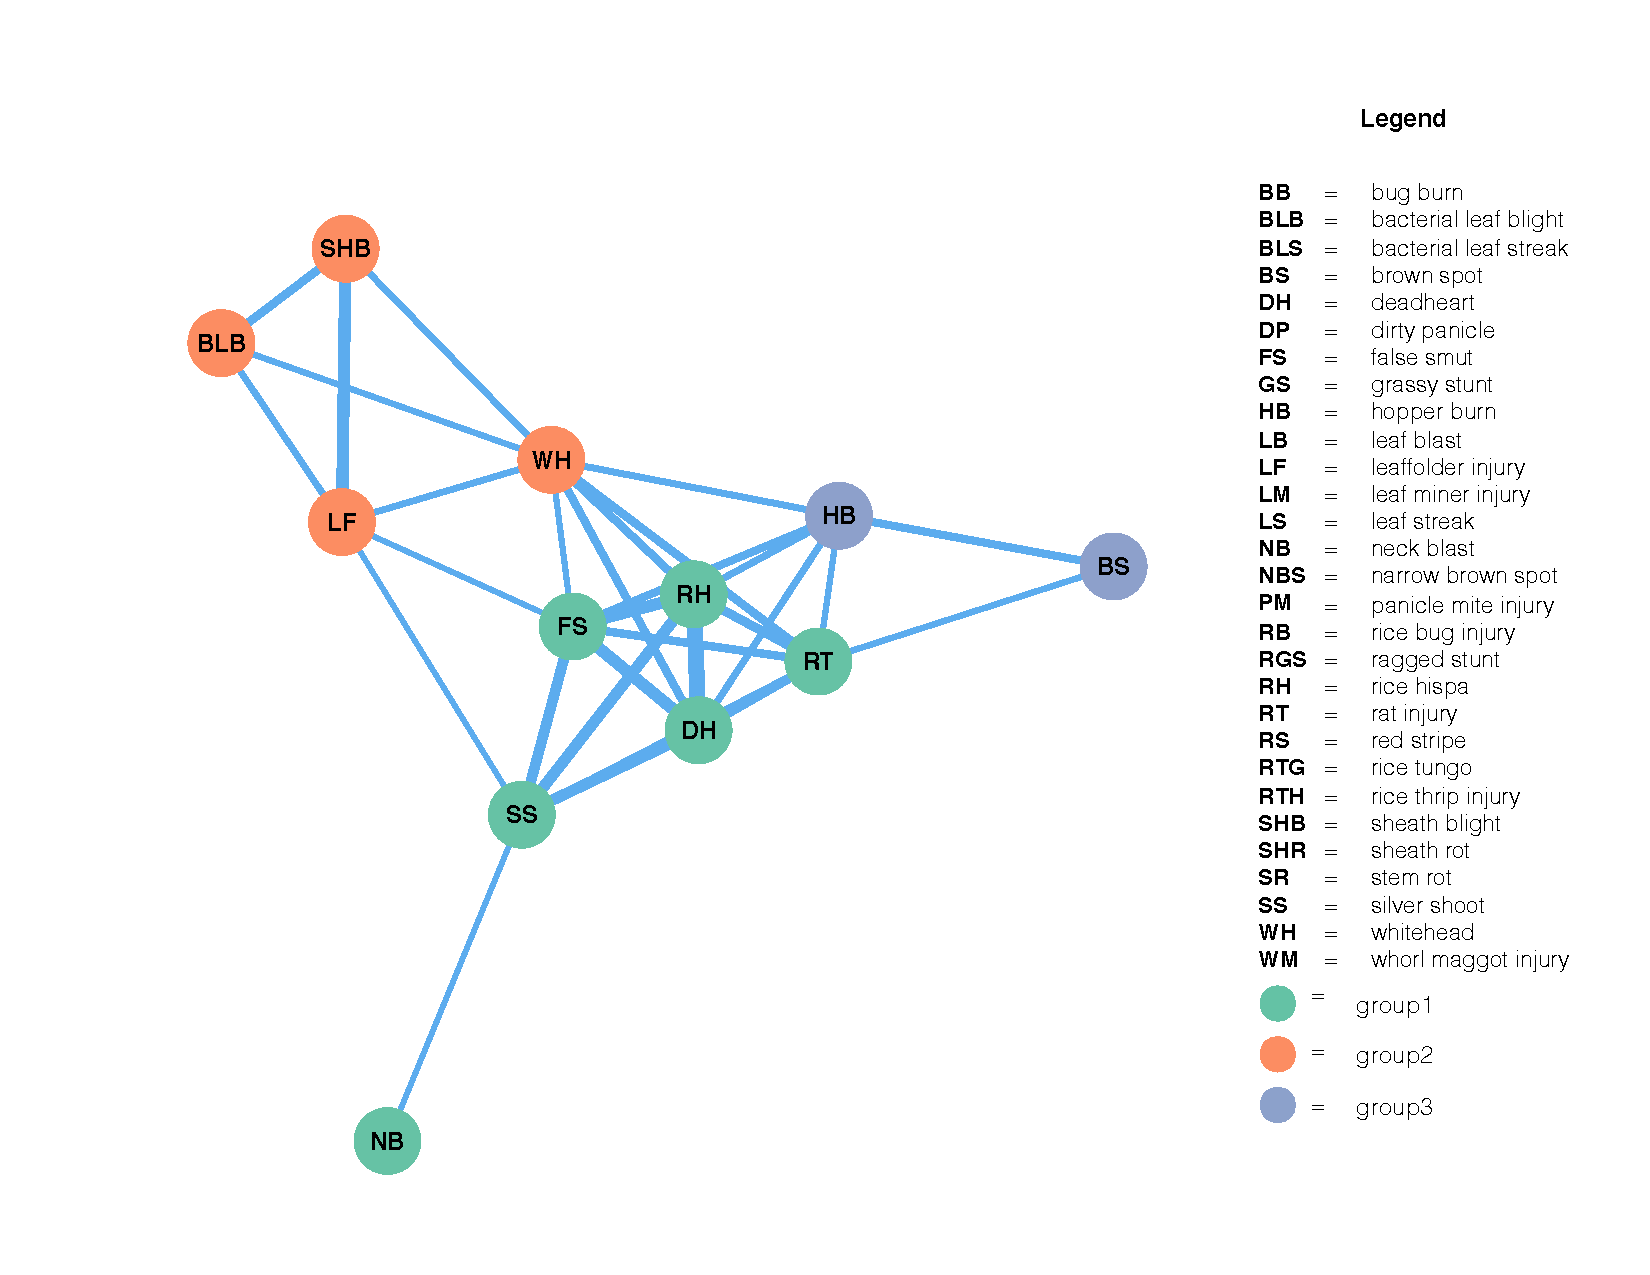
\includegraphics[width = 1\textwidth]{figures/networkTM_ws/networkTM_ws.pdf}
        \caption{Co-occurrence network of rice injuries in wet season at Tamil Nadu, India. The layout of the network graph is based on the Fruchterman-Reingold algorithm, which places nodes with stronger or more connections closer to each other.}
        \label{fig:networkTM_ws}
    \end{subfigure}
    \begin{subfigure}[b]{1\textwidth}
        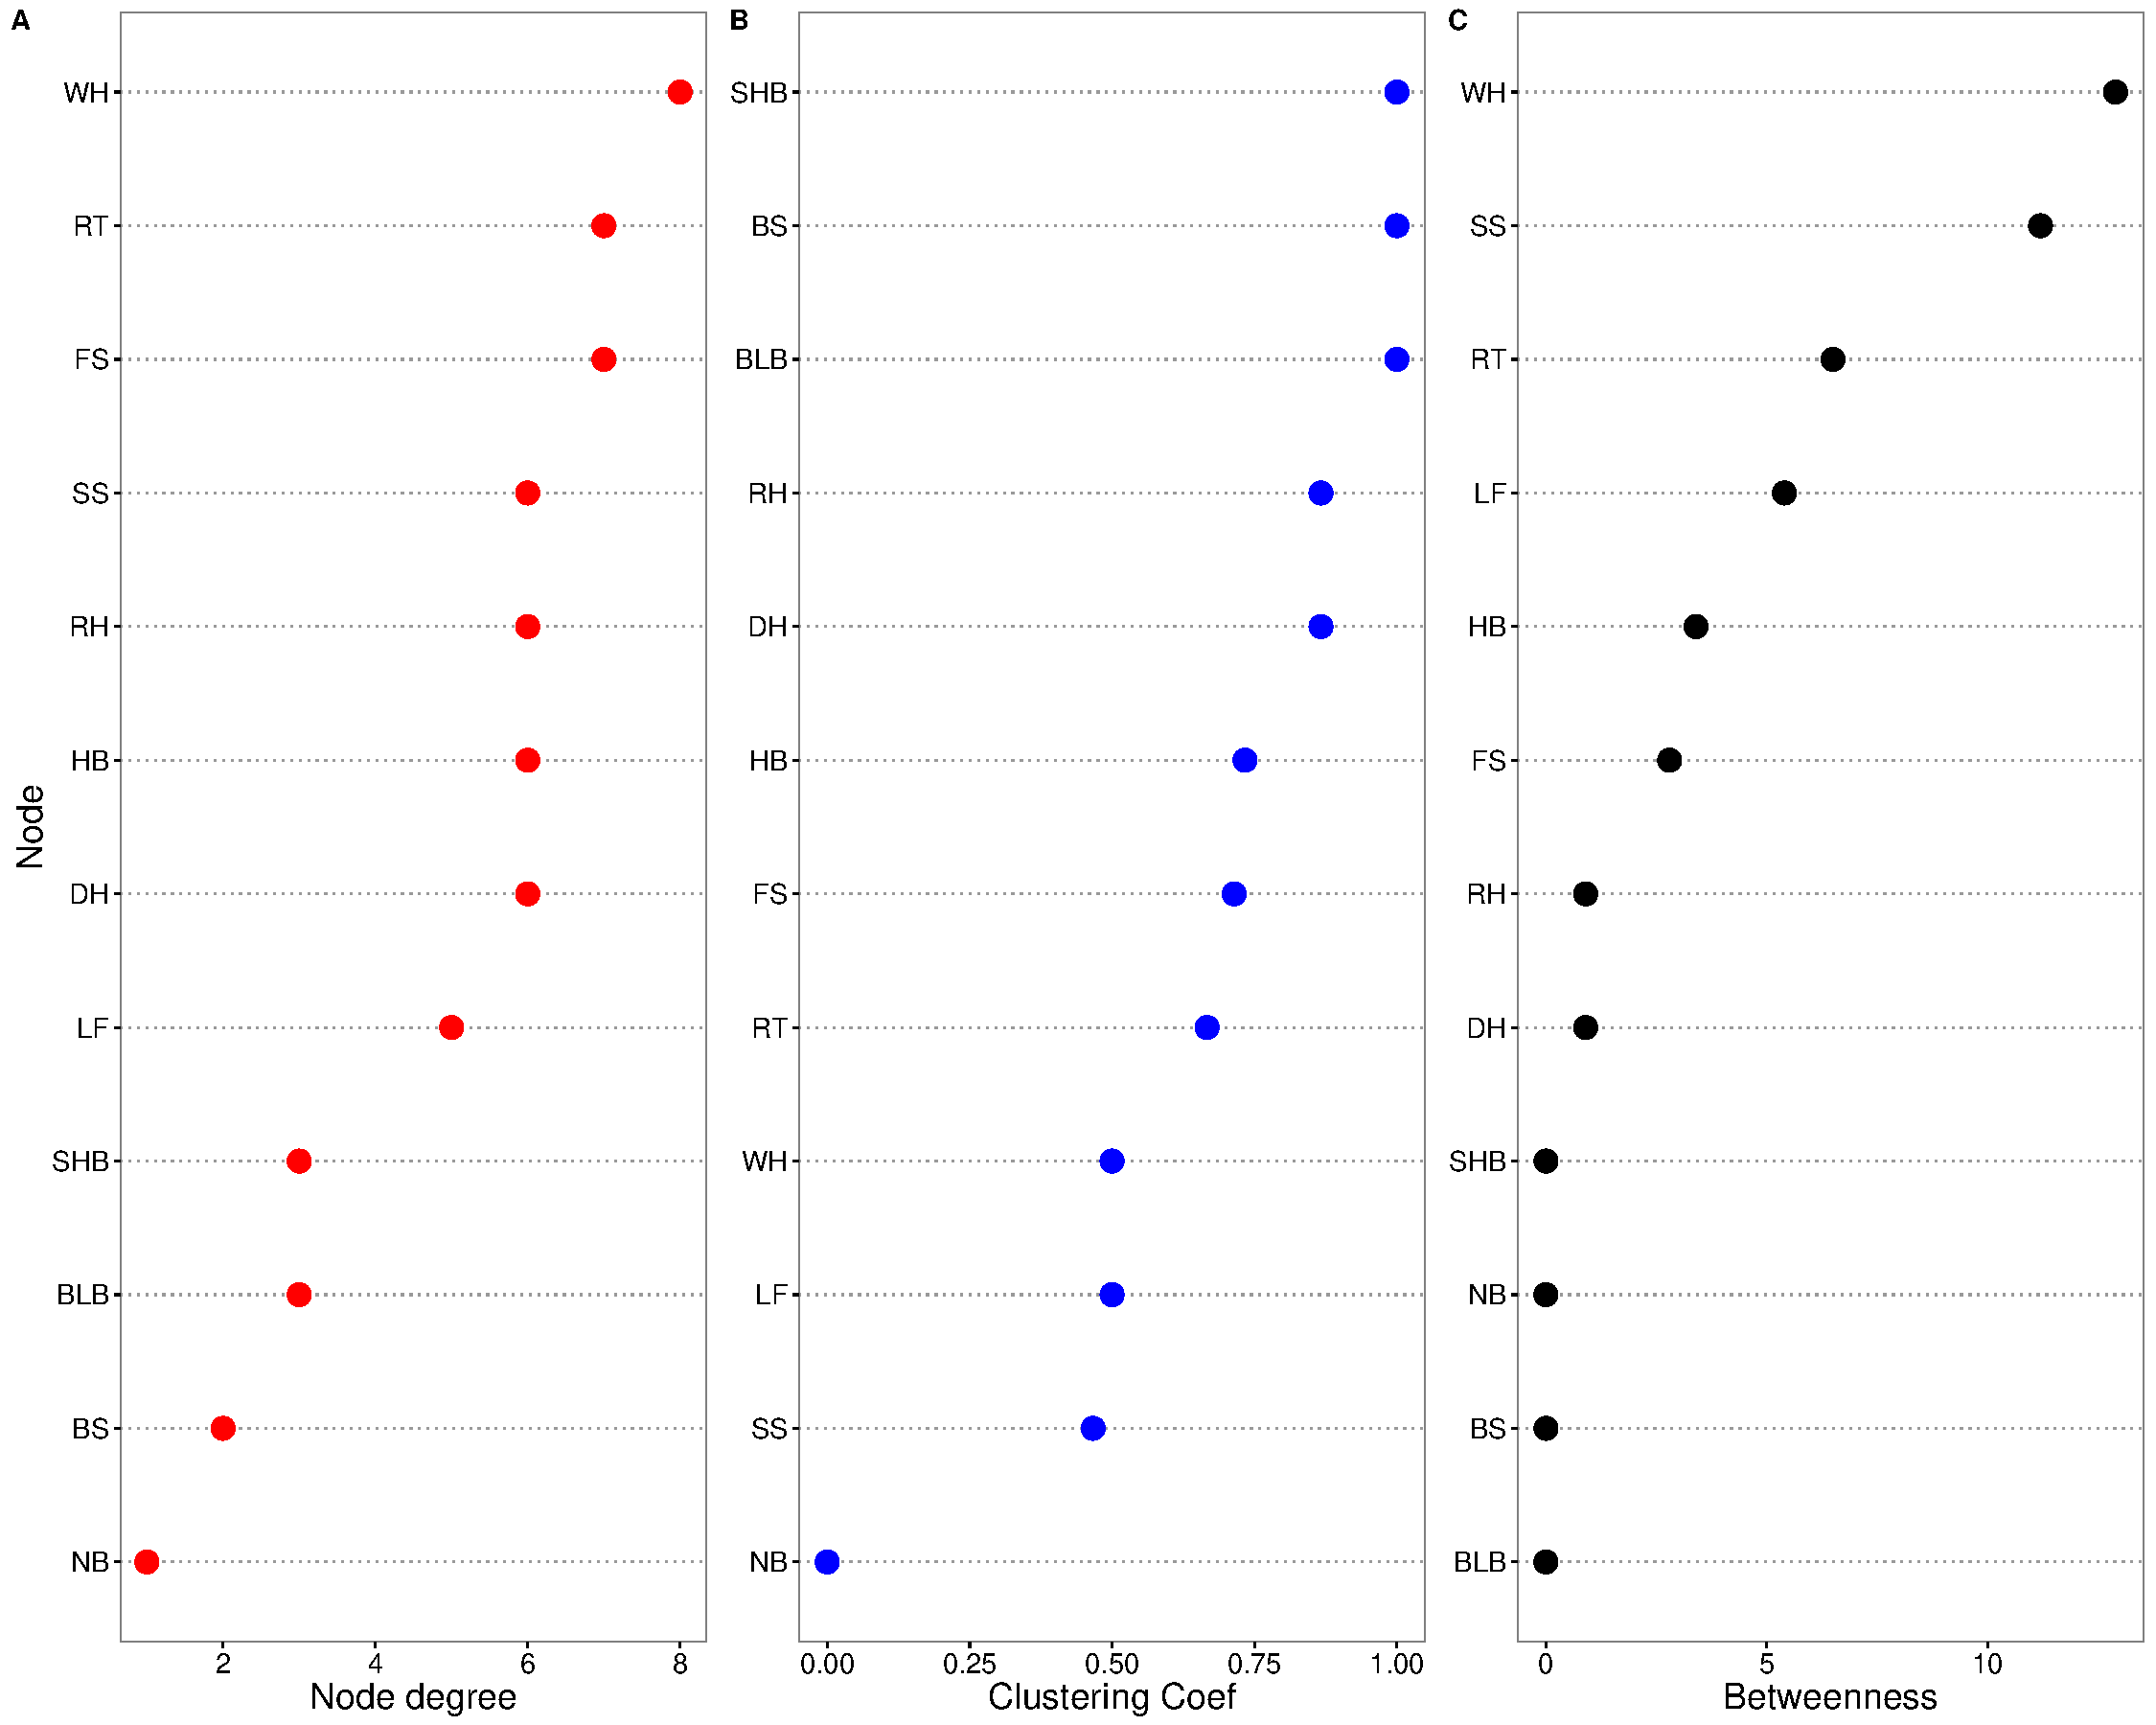
\includegraphics[width = 1\textwidth]{figures/nodepropTM_ws/nodepropTM_ws.pdf}
        \caption{Three centrality measures of the nodes in co-occurrence network of rice injuries in wet season at Tamil Nadu, India. A: node degree, B:clustering coefficient, and C:Betweenness, and.}
        \label{fig:nodepropTM_ws}
    \end{subfigure}
    \caption{Rice injuries in wet season in Tamil Nadu, India}
    \label{fig:TM_ws}
\end{figure}

\paragraph{West Java, Indonesia}

Co-occurrence network of injury profiles of dry season presented in Figure \ref{fig:networkWJ_ds}. The network reveals the four groups of injury profiles. Group1 (green) and group3 were close and group2 and group4 had less connection than others. Because of the structure and clustering coefficient, group1 and group3 are more likely to have chance to form association between the groups, and form complex association within group than between groups

Network in wet season (Figure \ref{fig:networkWJ_ws}) injuries and 54 associations. From the structure of this network, there were three type of injury syndromes.  One (group1; green) composed of SHB, RT, DH, RH, BLS, and SHR.  Within this group, BLS seems to be inducers (high betweenness), and SHB was connecter (high node degree). Two is combination of BS, LF, WM, NBS, and LM. This combination was clear that BS was dominant, and dominantly observed. Three is the combination of PM, RB, and FS. 

\begin{figure}
    \centering
    \begin{subfigure}[b]{1\textwidth}
        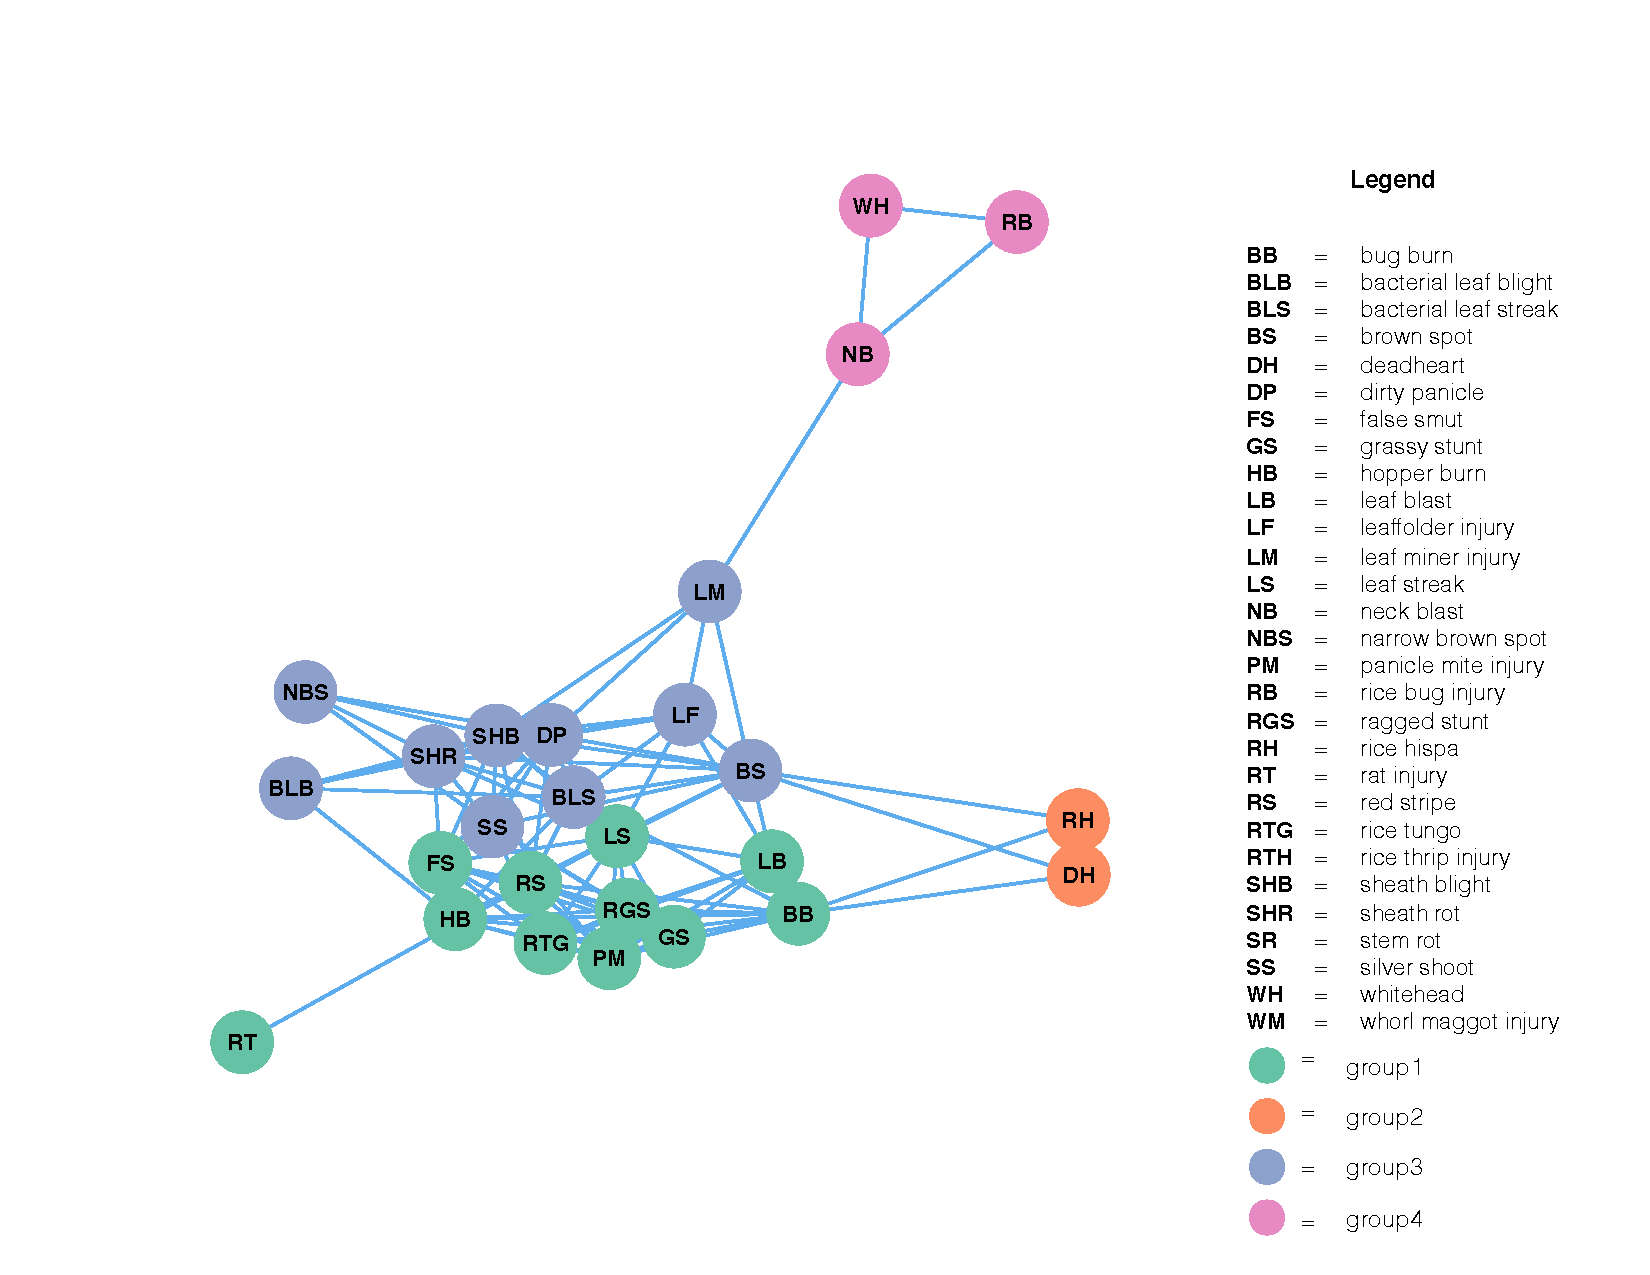
\includegraphics[width = 1\textwidth]{figures/networkWJ_ds/networkWJ_ds.pdf}
        \caption{Co-occurrence network of rice injuries in dry season at West Java, Indonesia. The layout of the network graph is based on the Fruchterman-Reingold algorithm, which places nodes with stronger or more connections closer to each other.}
        \label{fig:networkWJ_ds}
    \end{subfigure}
    \begin{subfigure}[b]{1\textwidth}
        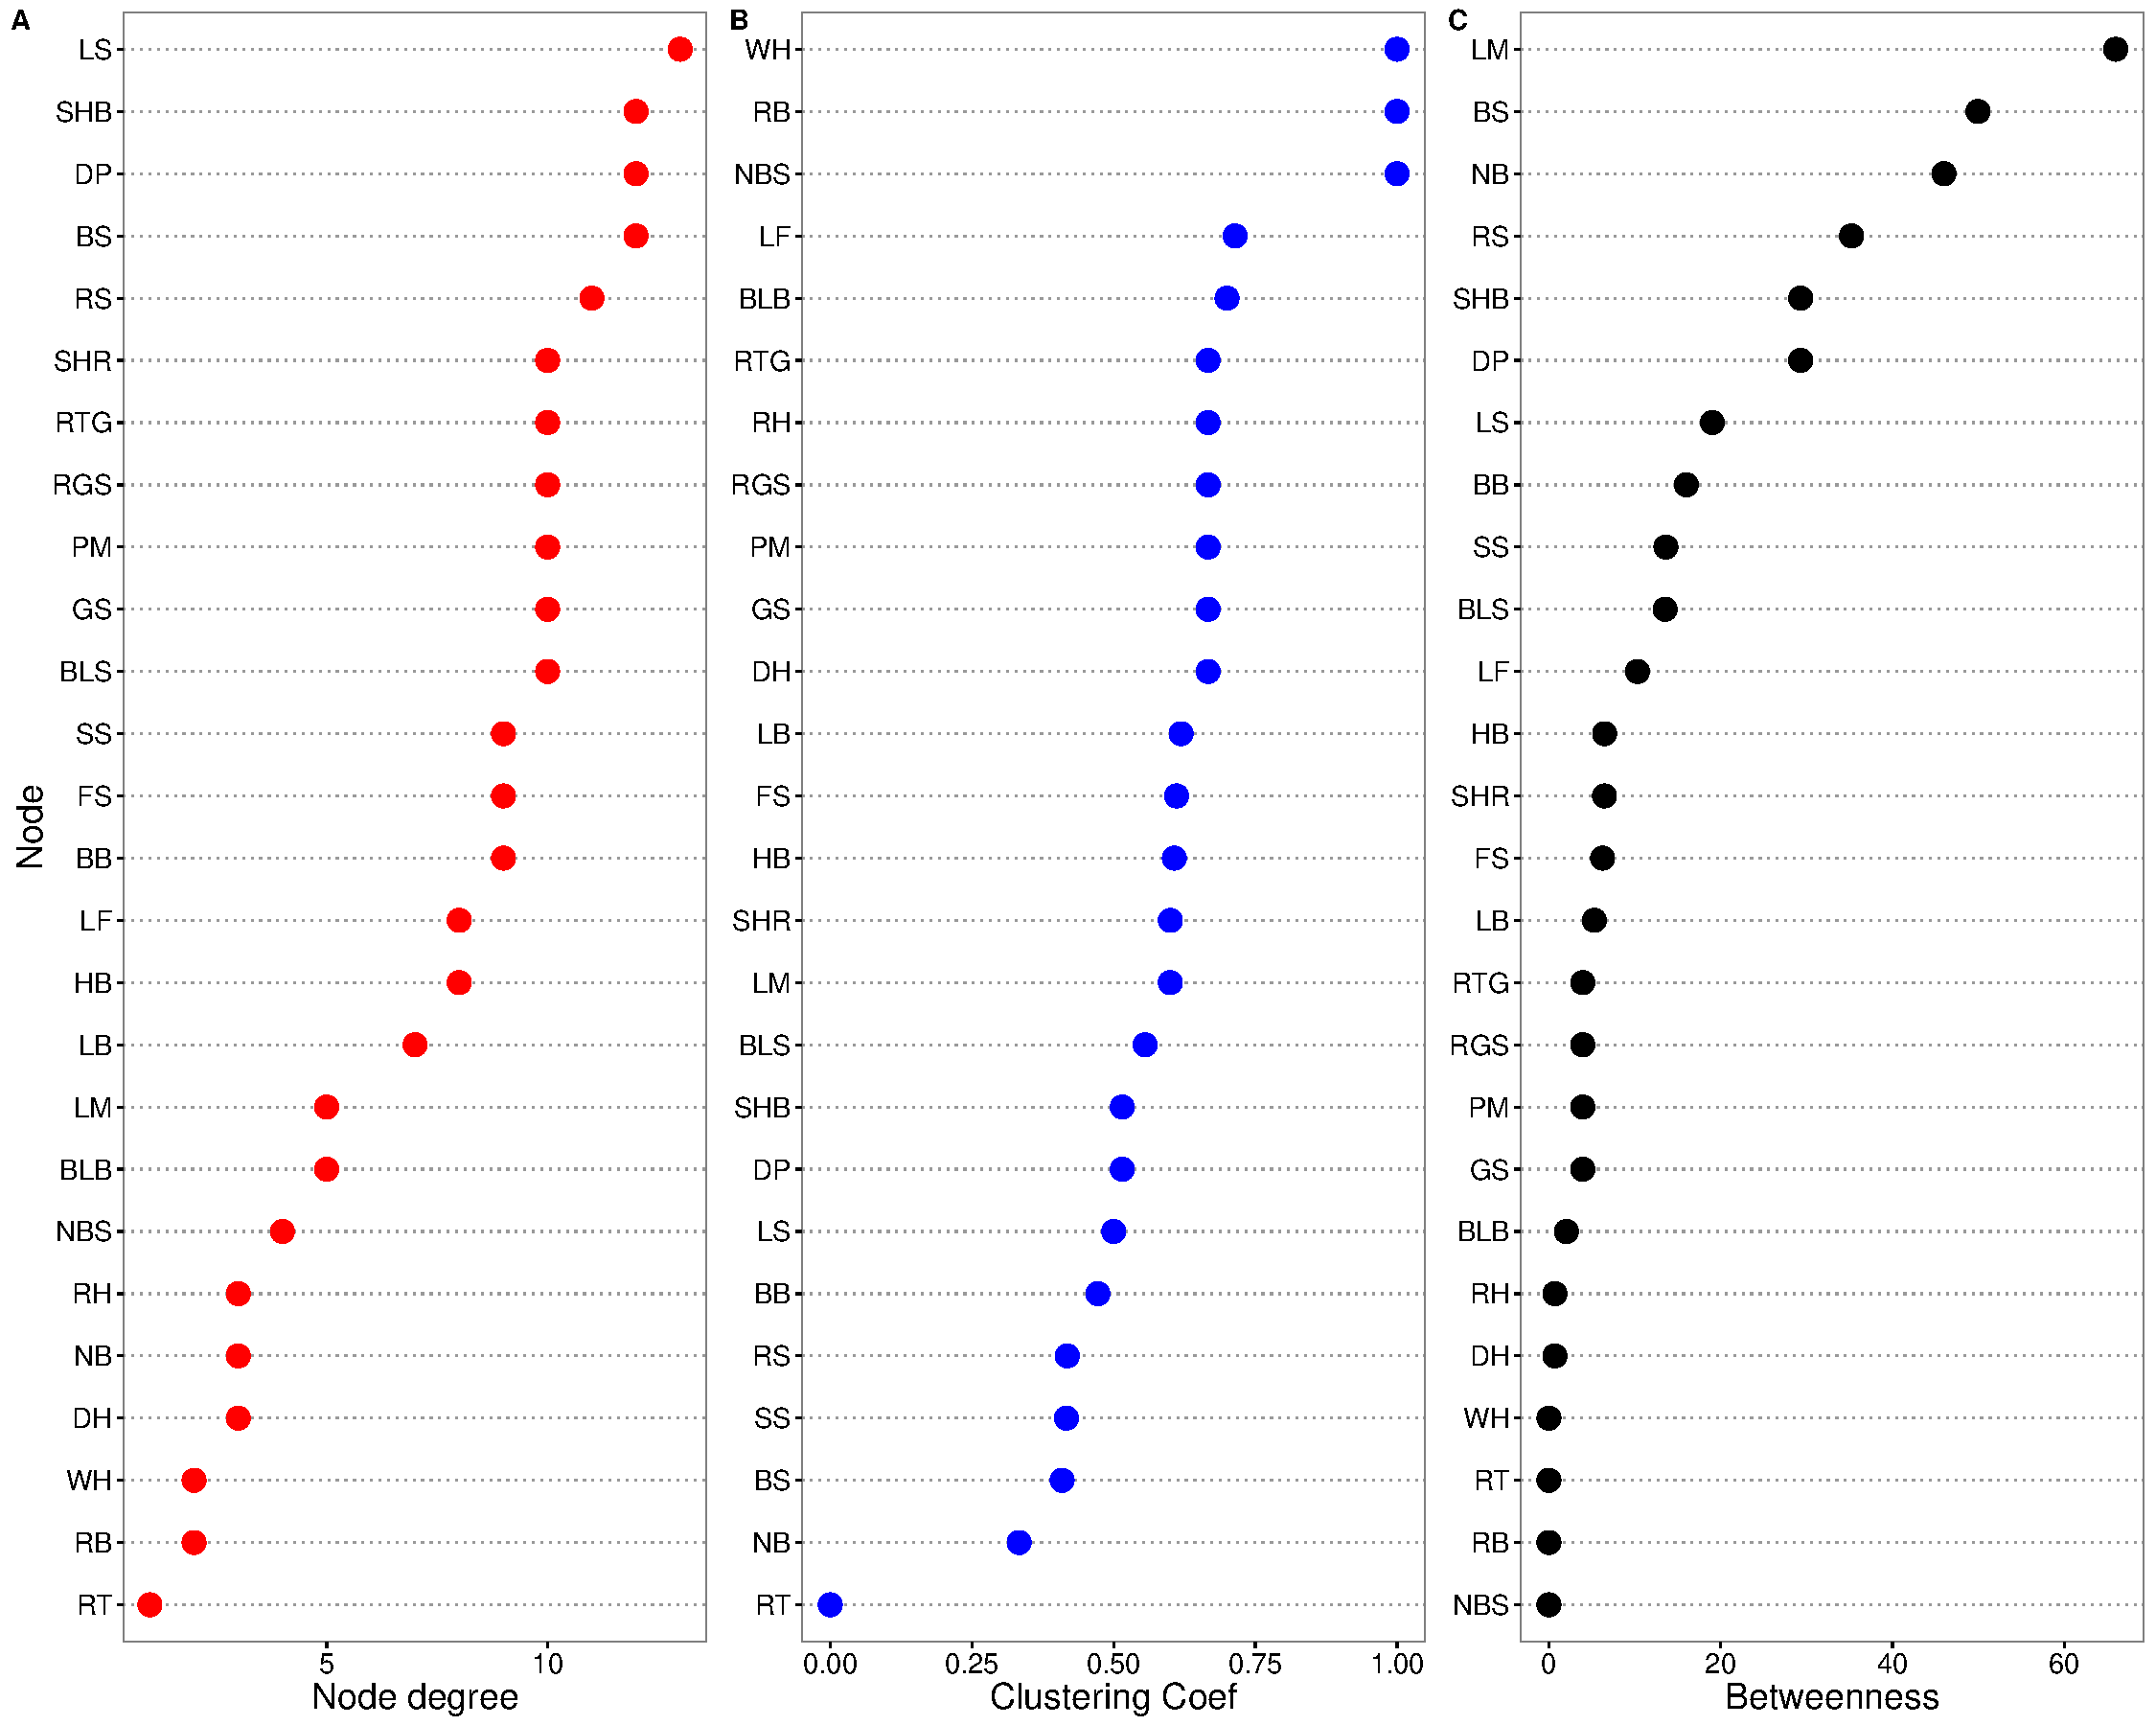
\includegraphics[width = 1\textwidth]{figures/nodepropWJ_ds/nodepropWJ_ds.pdf}
        \caption{Three centrality measures of the nodes in co-occurrence network of rice injuries in dry season at West Java, Indonesia. A: node degree, B:clustering coefficient, and C:Betweenness, and.}
        \label{fig:nodepropWJ_ds}
    \end{subfigure}
    \caption{Rice injuries in dry season in West Java, Indonesia}
    \label{fig:WJ_ds}
\end{figure}

\begin{figure}
    \centering
    \begin{subfigure}[b]{1\textwidth}
        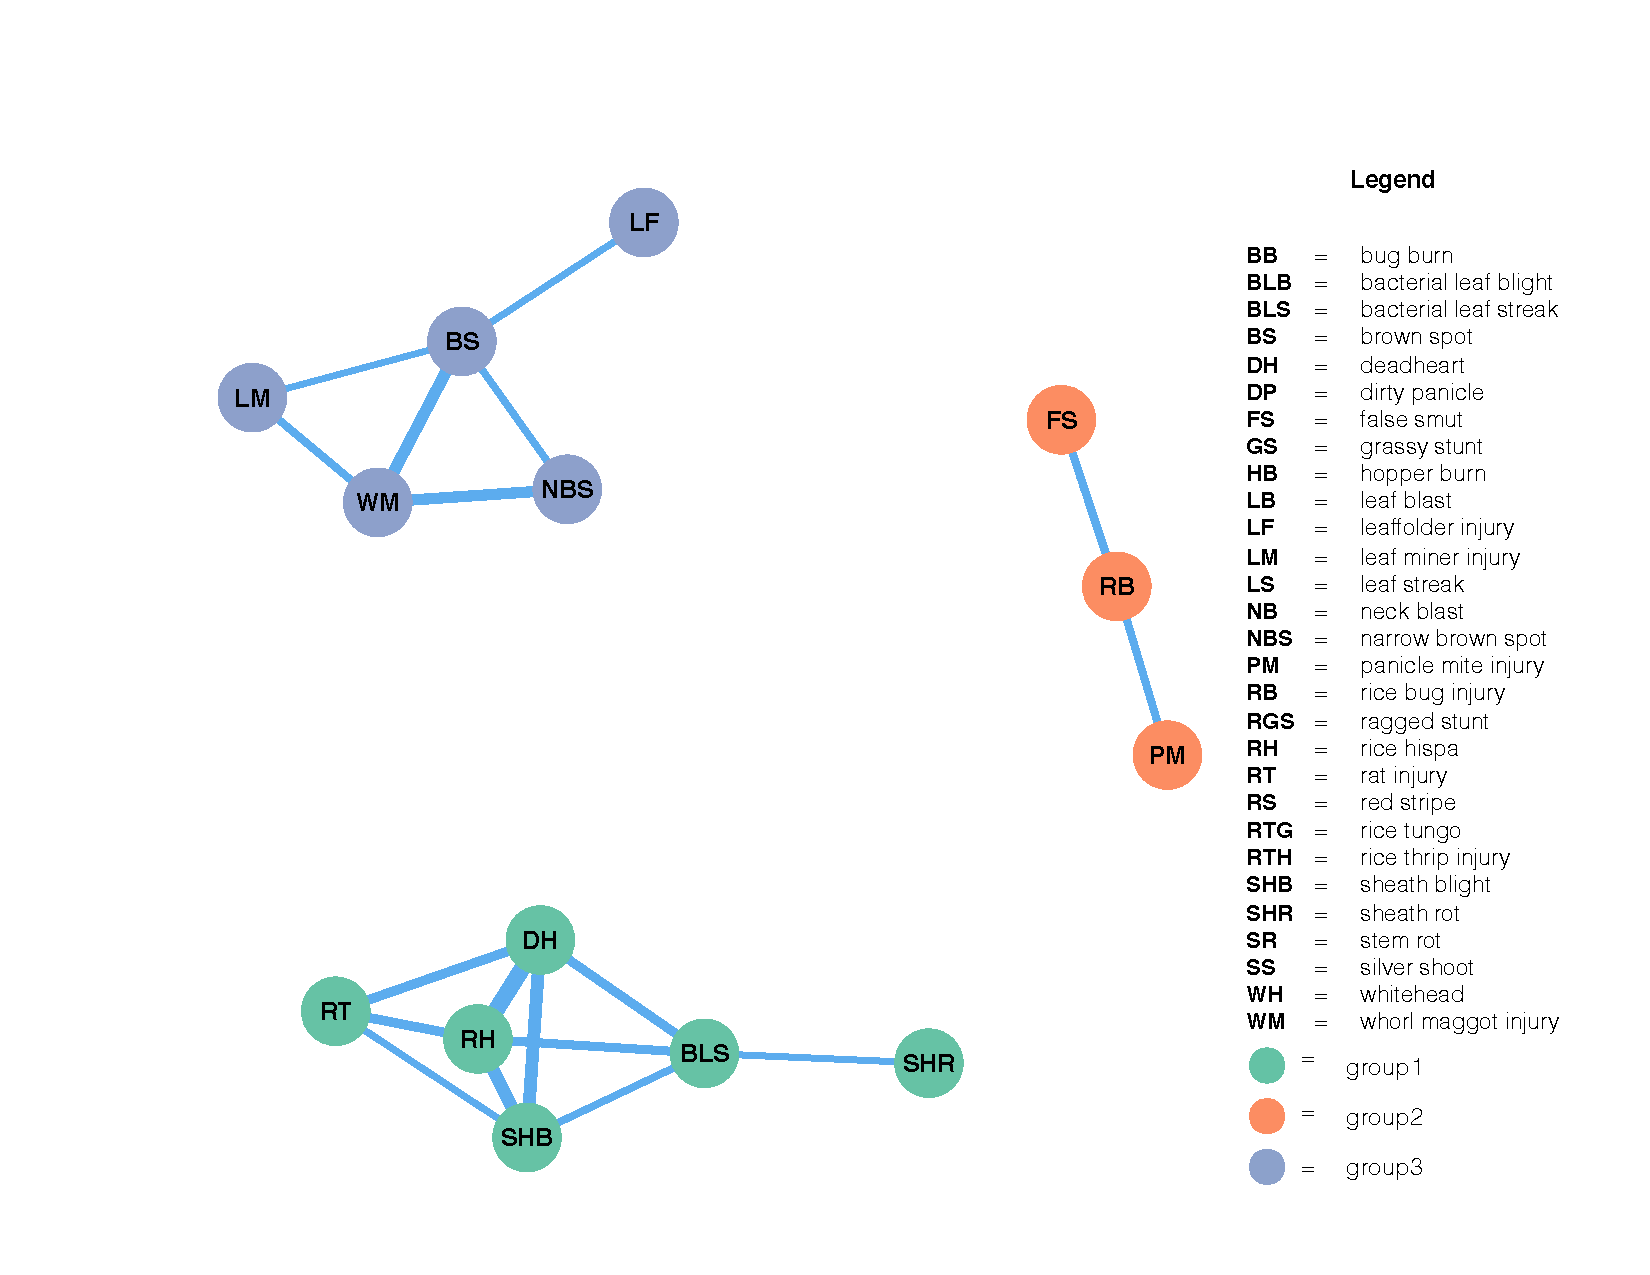
\includegraphics[width = 1\textwidth]{figures/networkWJ_ws/networkWJ_ws.pdf}
        \caption{Co-occurrence network of rice injuries in wet season at West Java, Indonesia. The layout of the network graph is based on the Fruchterman-Reingold algorithm, which places nodes with stronger or more connections closer to each other.}
        \label{fig:networkWJ_ws}
    \end{subfigure}
    \begin{subfigure}[b]{1\textwidth}
        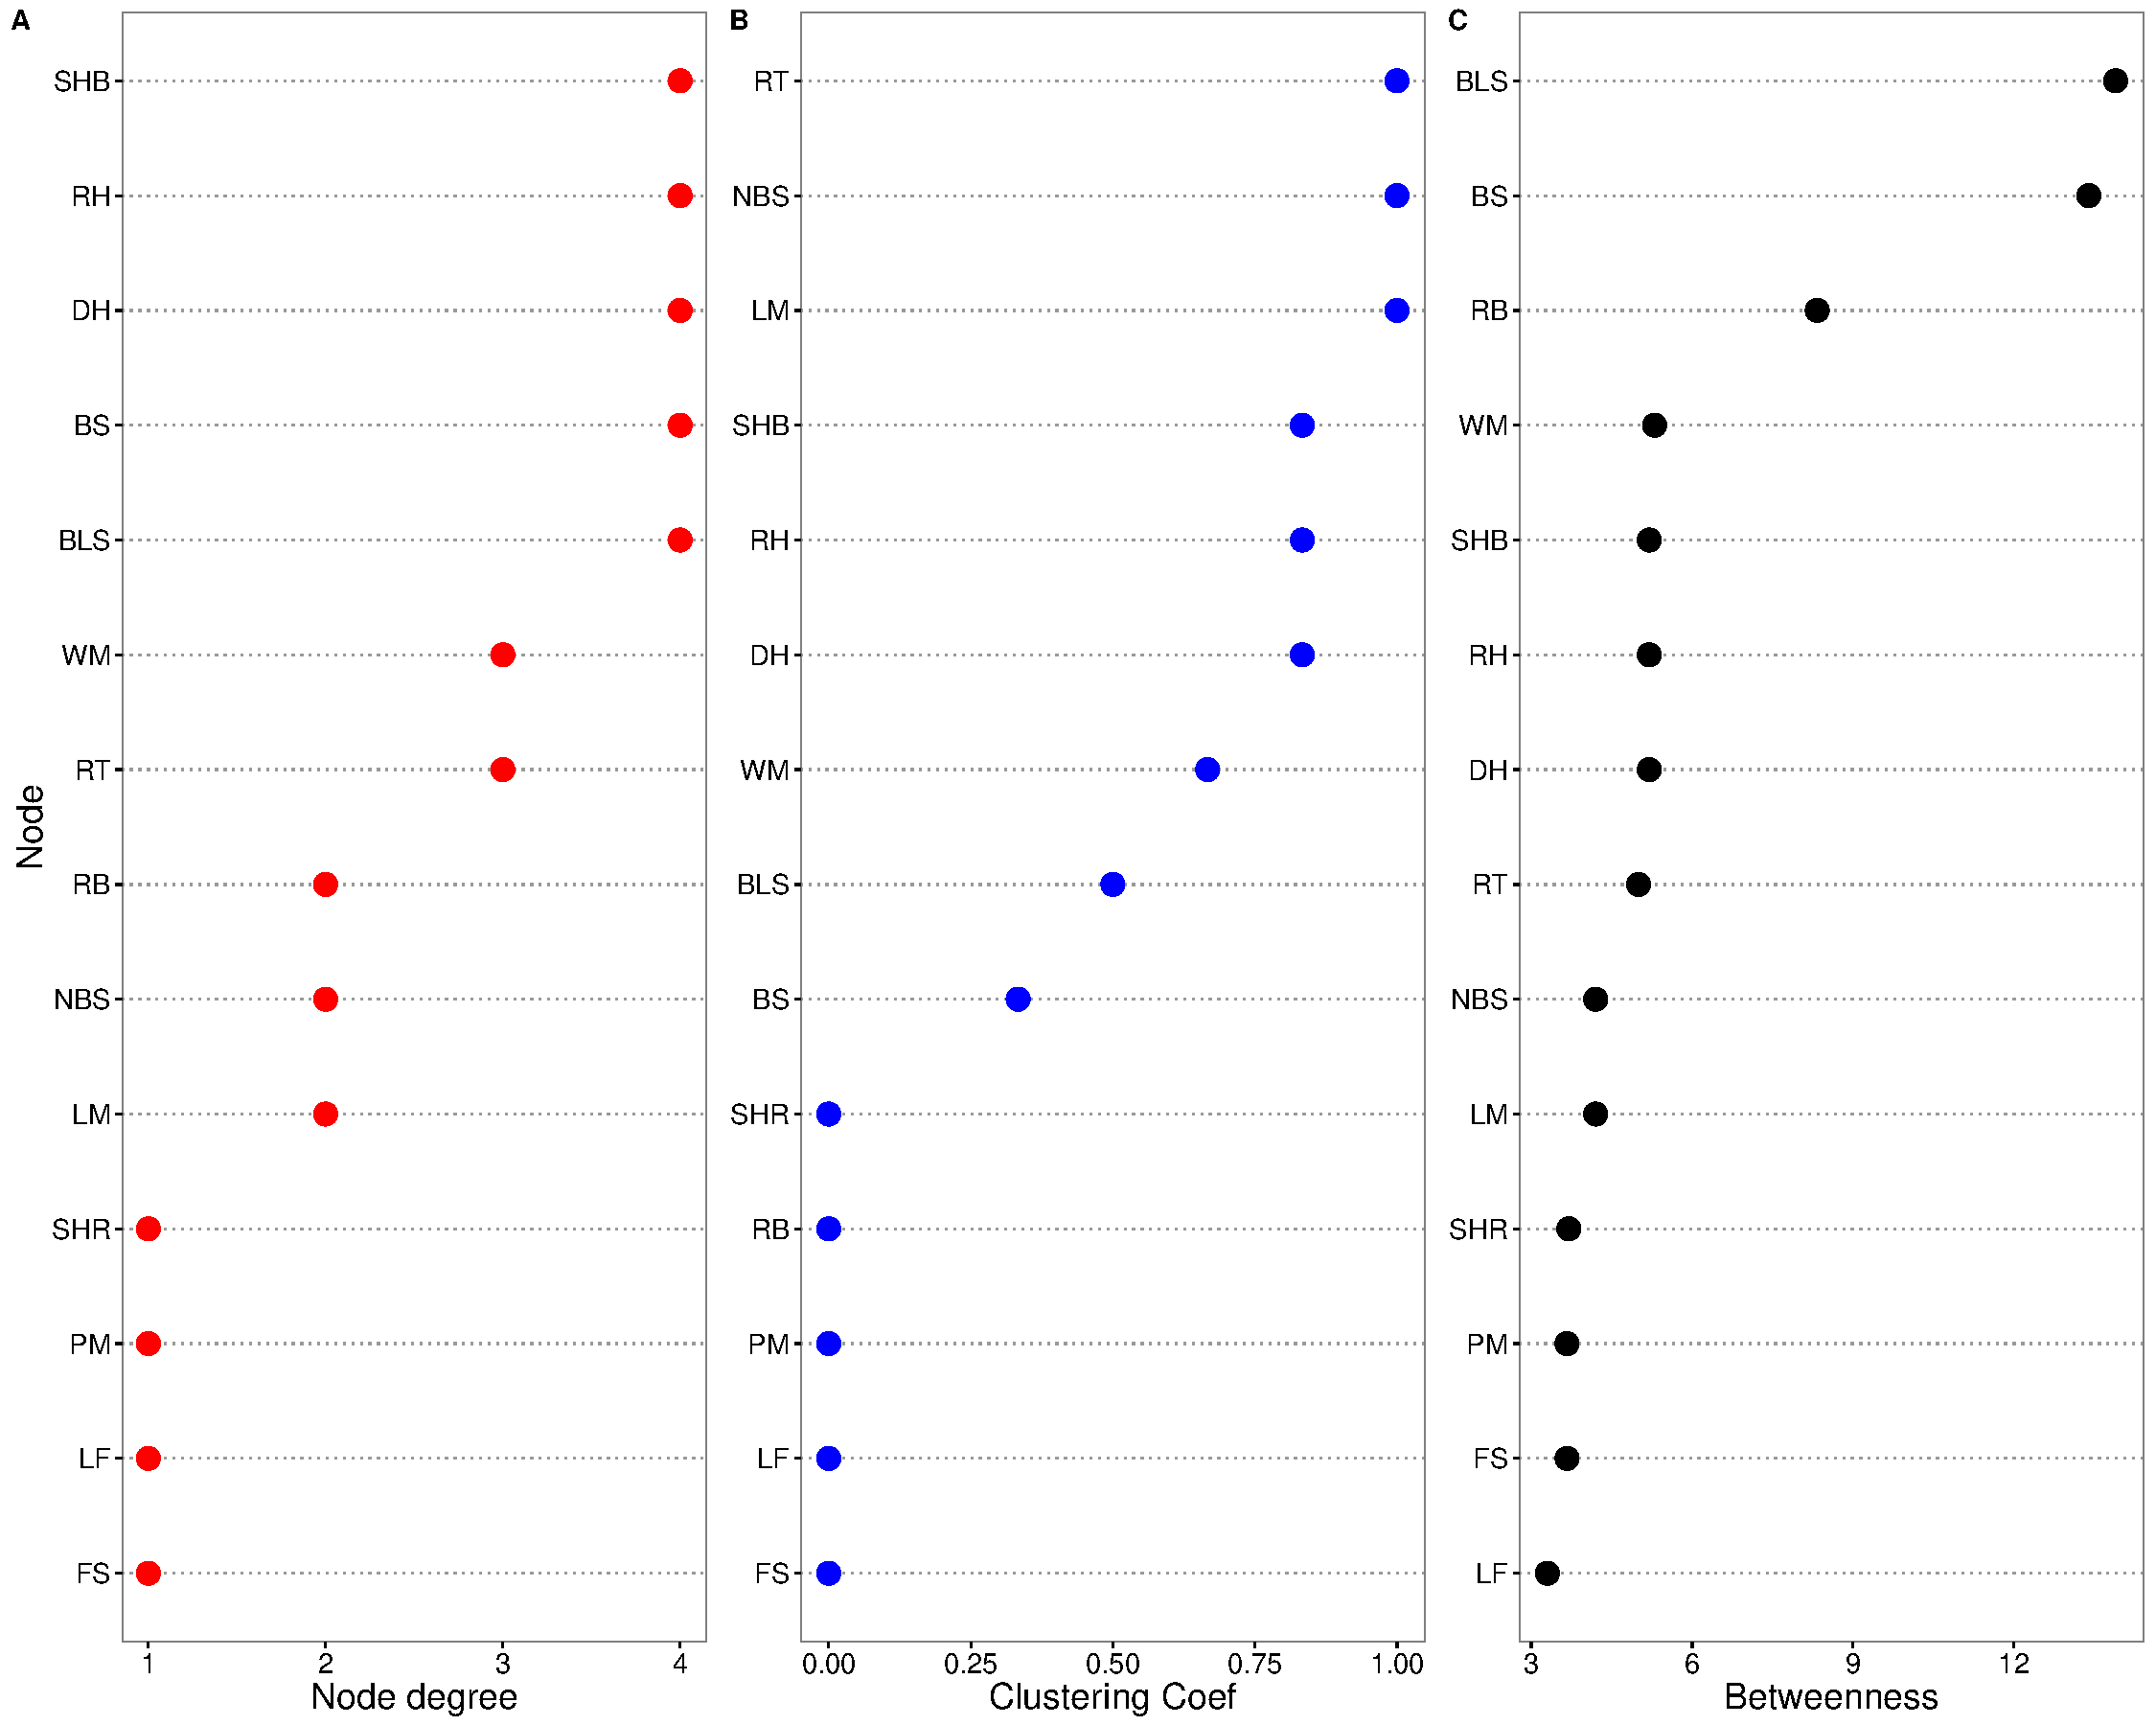
\includegraphics[width = 1\textwidth]{figures/nodepropWJ_ws/nodepropWJ_ws.pdf}
        \caption{Three centrality measures of the nodes in co-occurrence network of rice injuries in wet season at West Java, Indonesia. A: node degree, B:clustering coefficient, and C:Betweenness, and.}
        \label{fig:nodepropWJ_ds}
    \end{subfigure}
    \caption{Rice injuries in wet season in West Java, Indonesia}
    \label{fig:WJ_ws}
\end{figure}


\subsection{Discussion}
Even some nodes are less connected they may occuren in some season and not related to other and not fom co-ocurence

They may differul to preseict by suing other injuires 


Rice injuries were found commonly in South and South east Asia, but at different levels of incidence. 
Some injuries of this study is relatively low prevalence of areas that have been reported such as leaf blast, brown spot. It could be implied that these injuries strongly depended on locations or climatic conduction to develop, so they were not observed at all locations or seasons during survey were conducted. Another reason is that there are some factors such as the utility of resistance verities in the farmer’s fields surveyed, so we could observe those injuries at low level of incidence. The similar reasoning could explain to many injuries such as BLB, RB, NB, which widely occur in rice growing areas.

From the survey data of rice injuries observed in farmers’ fields, I analyzed the interaction and build the network based on that data. The methods applied for building a co-occurrence network of rice injuries were adapted from ecological studies. Usually, relationships were assessed using Pearson correlation. However, the use of the Pearson correlation coefficient is problematic because it requires the variables are applied with similar measure, and the variable values are normally distributed. Additionally, Pearson correlation can only capture linear relationships. Due to the fact that the assumptions of Pearson correlation are not fit with the survey data. The alternative is provided by using Spearman’s rank correlation coefficient, which is also widely used in ecological studies.

The exploration of co-occurrence networks is a useful method for determining interactions of co- occurring injuries. Network analysis has also suggested important injuries in networks. The important injuries were selected from the node features such as node degree, clustering coefficient, and betweenness. The betweenness represents the importance of the control potential that an injury exerts over the associations of other injuries in the network. The clustering coefficients are indicative of the potential spreading of the incidence of injuries through the network. As activated injury can activate other injuries, a more densely connected network facilitates injury activation \cite{Williams_2014_demonstrating}. In the network of dry season in West Java, Indonesia, BLB and SR can be the targets to be monitored because they have high betweenness, which indicated that they are more likely to present then others injuries.

It is good attempt to detect communities in a network because it can reveal information about the networks that is maybe not easy to detect by simple observation. The communities are groups of nodes that are densely connected among their node members, and slightly connected with the rest of the network.  In this study, we detected node community based on the optimization of the modularity of a sub-network, which is an approach that widely applied in many fields \cite{Liu_2014_Detecting}. Even though, the groups of injury profiles from this study are different from seasons and countries, but they are reasonable because some rice injuries present in some seasons (seasonal occurrence) such as gall midge injury \cite{Krishnaiah_2004_Rice}. The result also showed similar groups of injuries to the patterns of injuries profile from the study of \cite{Savary_2000_Characterization}. 

%SR is also best to be the target because it also associated with the RS, which has high clustering coefficients also because RS is potentially able to be co-found with many other injuries.  BLB also show the association with the injuries, which present high clustering coefficient. Both of BLB and SR are intermediate clustering coefficient., so they are formed concurrence between groups, but less potentially to present complex association. DH and WH are less associated with other injuries, so they are difficult to employ other injuries to. 

It is the good to monitored WM and RB  and SHB also even the GLH has no betweenness, but it has high clustering coefficients, and connected with two high betweenness node. It would be also good target to monitored also because when it present, it also frequency appear together.
We explored the characteristics of rice injury profiles

Communities are groups that are densely connected among their members, and sparsely connected with the rest of the network. Community structure can reveal abundant hidden information about complex networks that is not easy to detect by simple observation. 

With regard to pest management development, understanding that the relationships of rice injuries could simplify pest management decisions. As applied here, the node degree, clustering coefficients, and betweenness described the interaction of injuries in the networks. Therefore, they may be useful in finding a good indicator for monitoring pest in rice fields. High-betweenness node High- clustering coefficient node 

Community structure in complex network can reveal hidden information about complex networks that is maybe not easy to detect by simple observation such as nodes, which are clustered. In this study, we detected node community based on the optimization of the modularity of a sub-network, which is a popular approach \cite{Liu_2014_Detecting}. Even though, the groups of injury profiles from this study are different from seasons and countries, but they are reasonable because some rice injuries present in some seasons (seasonal occurrence) such as gall midge injury \cite{Krishnaiah_2004_Rice}. from the groups of injury profile from \cite{Savary_2000_Characterization}. 



\subsection{Conclusion}

